\documentclass{book}
\usepackage[a4paper,top=2.5cm,bottom=2.5cm,left=2.5cm,right=2.5cm]{geometry}
\usepackage{makeidx}
\usepackage{natbib}
\usepackage{graphicx}
\usepackage{multicol}
\usepackage{float}
\usepackage{listings}
\usepackage{color}
\usepackage{ifthen}
\usepackage[table]{xcolor}
\usepackage{textcomp}
\usepackage{alltt}
\usepackage{ifpdf}
\ifpdf
\usepackage[pdftex,
            pagebackref=true,
            colorlinks=true,
            linkcolor=blue,
            unicode
           ]{hyperref}
\else
\usepackage[ps2pdf,
            pagebackref=true,
            colorlinks=true,
            linkcolor=blue,
            unicode
           ]{hyperref}
\usepackage{pspicture}
\fi
\usepackage[utf8]{inputenc}
\usepackage{mathptmx}
\usepackage[scaled=.90]{helvet}
\usepackage{courier}
\usepackage{sectsty}
\usepackage{amssymb}
\usepackage[titles]{tocloft}
\usepackage{doxygen}
\lstset{language=C++,inputencoding=utf8,basicstyle=\footnotesize,breaklines=true,breakatwhitespace=true,tabsize=4,numbers=left }
\makeindex
\setcounter{tocdepth}{3}
\renewcommand{\footrulewidth}{0.4pt}
\renewcommand{\familydefault}{\sfdefault}
\hfuzz=15pt
\setlength{\emergencystretch}{15pt}
\hbadness=750
\tolerance=750
\begin{document}
\hypersetup{pageanchor=false,citecolor=blue}
\begin{titlepage}
\vspace*{7cm}
\begin{center}
{\Large Fluid Survival Tool \\[1ex]\large 0.\-03 }\\
\vspace*{1cm}
{\large Generated by Doxygen 1.8.3.1}\\
\vspace*{0.5cm}
{\small Mon Jun 24 2013 16:58:31}\\
\end{center}
\end{titlepage}
\clearemptydoublepage
\pagenumbering{roman}
\tableofcontents
\clearemptydoublepage
\pagenumbering{arabic}
\hypersetup{pageanchor=true,citecolor=blue}
\chapter{Hierarchical Index}
\section{Class Hierarchy}
This inheritance list is sorted roughly, but not completely, alphabetically\-:\begin{DoxyCompactList}
\item \contentsline{section}{model\-:\-:Arc}{\pageref{structmodel_1_1Arc}}{}
\item \contentsline{section}{Clipper\-Lib\-:\-:Clipper\-Base}{\pageref{classClipperLib_1_1ClipperBase}}{}
\begin{DoxyCompactList}
\item \contentsline{section}{Clipper\-Lib\-:\-:Clipper}{\pageref{classClipperLib_1_1Clipper}}{}
\end{DoxyCompactList}
\item \contentsline{section}{Clipper\-Lib\-:\-:Double\-Point}{\pageref{structClipperLib_1_1DoublePoint}}{}
\item \contentsline{section}{model\-:\-:Dtrm\-Event}{\pageref{structmodel_1_1DtrmEvent}}{}
\item exception\begin{DoxyCompactList}
\item \contentsline{section}{Clipper\-Lib\-:\-:clipper\-Exception}{\pageref{classClipperLib_1_1clipperException}}{}
\end{DoxyCompactList}
\item \contentsline{section}{model\-:\-:Facade}{\pageref{classmodel_1_1Facade}}{}
\item \contentsline{section}{model\-:\-:Formula}{\pageref{classmodel_1_1Formula}}{}
\begin{DoxyCompactList}
\item \contentsline{section}{model\-:\-:A\-D\-Formula}{\pageref{classmodel_1_1ADFormula}}{}
\item \contentsline{section}{model\-:\-:A\-D\-Formula}{\pageref{classmodel_1_1ADFormula}}{}
\item \contentsline{section}{model\-:\-:And\-Formula}{\pageref{classmodel_1_1AndFormula}}{}
\item \contentsline{section}{model\-:\-:And\-Formula}{\pageref{classmodel_1_1AndFormula}}{}
\item \contentsline{section}{model\-:\-:Atom\-Cont\-Formula}{\pageref{classmodel_1_1AtomContFormula}}{}
\item \contentsline{section}{model\-:\-:Atom\-Cont\-Formula}{\pageref{classmodel_1_1AtomContFormula}}{}
\item \contentsline{section}{model\-:\-:Atom\-Dis\-Formula}{\pageref{classmodel_1_1AtomDisFormula}}{}
\item \contentsline{section}{model\-:\-:Atom\-Dis\-Formula}{\pageref{classmodel_1_1AtomDisFormula}}{}
\item \contentsline{section}{model\-:\-:Neg\-Formula}{\pageref{classmodel_1_1NegFormula}}{}
\item \contentsline{section}{model\-:\-:Neg\-Formula}{\pageref{classmodel_1_1NegFormula}}{}
\item \contentsline{section}{model\-:\-:Prob\-Formula}{\pageref{classmodel_1_1ProbFormula}}{}
\item \contentsline{section}{model\-:\-:Prob\-Formula}{\pageref{classmodel_1_1ProbFormula}}{}
\item \contentsline{section}{model\-:\-:True\-Formula}{\pageref{classmodel_1_1TrueFormula}}{}
\item \contentsline{section}{model\-:\-:True\-Formula}{\pageref{classmodel_1_1TrueFormula}}{}
\item \contentsline{section}{model\-:\-:Until\-Formula}{\pageref{classmodel_1_1UntilFormula}}{}
\item \contentsline{section}{model\-:\-:Until\-Formula}{\pageref{classmodel_1_1UntilFormula}}{}
\end{DoxyCompactList}
\item \contentsline{section}{Formula}{\pageref{structFormula}}{}
\item \contentsline{section}{model\-:\-:Geometry\-Helper}{\pageref{classmodel_1_1GeometryHelper}}{}
\item \contentsline{section}{Clipper\-Lib\-:\-:Horz\-Join\-Rec}{\pageref{structClipperLib_1_1HorzJoinRec}}{}
\item \contentsline{section}{Clipper\-Lib\-:\-:Int128}{\pageref{classClipperLib_1_1Int128}}{}
\item \contentsline{section}{Clipper\-Lib\-:\-:Intersect\-Node}{\pageref{structClipperLib_1_1IntersectNode}}{}
\item \contentsline{section}{Interval}{\pageref{structInterval}}{}
\item \contentsline{section}{model\-:\-:Interval}{\pageref{classmodel_1_1Interval}}{}
\item \contentsline{section}{model\-:\-:Interval\-Set}{\pageref{classmodel_1_1IntervalSet}}{}
\item \contentsline{section}{Clipper\-Lib\-:\-:Int\-Point}{\pageref{structClipperLib_1_1IntPoint}}{}
\item \contentsline{section}{Clipper\-Lib\-:\-:Int\-Rect}{\pageref{structClipperLib_1_1IntRect}}{}
\item \contentsline{section}{Clipper\-Lib\-:\-:Join\-Rec}{\pageref{structClipperLib_1_1JoinRec}}{}
\item \contentsline{section}{model\-:\-:Line}{\pageref{classmodel_1_1Line}}{}
\begin{DoxyCompactList}
\item \contentsline{section}{model\-:\-:Segment}{\pageref{classmodel_1_1Segment}}{}
\end{DoxyCompactList}
\item \contentsline{section}{Clipper\-Lib\-:\-:Local\-Minima}{\pageref{structClipperLib_1_1LocalMinima}}{}
\item \contentsline{section}{model\-:\-:location}{\pageref{classmodel_1_1location}}{}
\item \contentsline{section}{model\-:\-:Logger}{\pageref{classmodel_1_1Logger}}{}
\begin{DoxyCompactList}
\item \contentsline{section}{G\-U\-I\-Controller}{\pageref{classGUIController}}{}
\end{DoxyCompactList}
\item \contentsline{section}{model\-:\-:Marking}{\pageref{structmodel_1_1Marking}}{}
\item \contentsline{section}{model\-:\-:min\-List}{\pageref{structmodel_1_1minList}}{}
\item \contentsline{section}{model\-:\-:Model}{\pageref{structmodel_1_1Model}}{}
\item \contentsline{section}{model\-:\-:Model\-Checker}{\pageref{classmodel_1_1ModelChecker}}{}
\item \contentsline{section}{Clipper\-Lib\-:\-:Out\-Pt}{\pageref{structClipperLib_1_1OutPt}}{}
\item \contentsline{section}{Clipper\-Lib\-:\-:Out\-Rec}{\pageref{structClipperLib_1_1OutRec}}{}
\item \contentsline{section}{model\-:\-:Place}{\pageref{structmodel_1_1Place}}{}
\item \contentsline{section}{model\-:\-:Point}{\pageref{structmodel_1_1Point}}{}
\item \contentsline{section}{model\-:\-:Polygon}{\pageref{classmodel_1_1Polygon}}{}
\item \contentsline{section}{Clipper\-Lib\-:\-:Poly\-Node}{\pageref{classClipperLib_1_1PolyNode}}{}
\begin{DoxyCompactList}
\item \contentsline{section}{Clipper\-Lib\-:\-:Poly\-Tree}{\pageref{classClipperLib_1_1PolyTree}}{}
\end{DoxyCompactList}
\item \contentsline{section}{Clipper\-Lib\-:\-:Poly\-Offset\-Builder}{\pageref{classClipperLib_1_1PolyOffsetBuilder}}{}
\item \contentsline{section}{model\-:\-:position}{\pageref{classmodel_1_1position}}{}
\item Q\-Dialog\begin{DoxyCompactList}
\item \contentsline{section}{Model\-Check\-Dialog\-Controller}{\pageref{classModelCheckDialogController}}{}
\item \contentsline{section}{Place\-Prob\-Dialog\-Controller}{\pageref{classPlaceProbDialogController}}{}
\item \contentsline{section}{S\-T\-D\-Dialog\-Controller}{\pageref{classSTDDialogController}}{}
\end{DoxyCompactList}
\item Q\-Main\-Window\begin{DoxyCompactList}
\item \contentsline{section}{G\-U\-I\-Controller}{\pageref{classGUIController}}{}
\item \contentsline{section}{G\-U\-I\-Controller}{\pageref{classGUIController}}{}
\end{DoxyCompactList}
\item \contentsline{section}{model\-:\-:Region}{\pageref{classmodel_1_1Region}}{}
\item \contentsline{section}{Clipper\-Lib\-:\-:Scanbeam}{\pageref{structClipperLib_1_1Scanbeam}}{}
\item \contentsline{section}{model\-:\-:slice$<$ T, S $>$}{\pageref{classmodel_1_1slice}}{}
\item \contentsline{section}{model\-:\-:stack$<$ T, S $>$}{\pageref{classmodel_1_1stack}}{}
\item \contentsline{section}{model\-:\-:State\-\_\-tag}{\pageref{structmodel_1_1State__tag}}{}
\item \contentsline{section}{model\-:\-:State\-Prob\-Alt\-\_\-tag}{\pageref{structmodel_1_1StateProbAlt__tag}}{}
\item \contentsline{section}{model\-:\-:State\-Time\-Alt\-\_\-tag}{\pageref{structmodel_1_1StateTimeAlt__tag}}{}
\item \contentsline{section}{model\-:\-:Stochastic\-Event}{\pageref{structmodel_1_1StochasticEvent}}{}
\item \contentsline{section}{Clipper\-Lib\-:\-:T\-Edge}{\pageref{structClipperLib_1_1TEdge}}{}
\item \contentsline{section}{model\-:\-:Timed\-Diagram}{\pageref{classmodel_1_1TimedDiagram}}{}
\item \contentsline{section}{Token}{\pageref{structToken}}{}
\item \contentsline{section}{model\-:\-:Transition}{\pageref{structmodel_1_1Transition}}{}
\item \contentsline{section}{yy\-\_\-buffer\-\_\-state}{\pageref{structyy__buffer__state}}{}
\item \contentsline{section}{yy\-\_\-trans\-\_\-info}{\pageref{structyy__trans__info}}{}
\item \contentsline{section}{yyalloc}{\pageref{unionyyalloc}}{}
\item \contentsline{section}{Y\-Y\-M\-I\-N\-O\-R\-T\-Y\-P\-E}{\pageref{unionYYMINORTYPE}}{}
\item \contentsline{section}{yy\-Parser}{\pageref{structyyParser}}{}
\item \contentsline{section}{yy\-Stack\-Entry}{\pageref{structyyStackEntry}}{}
\item \contentsline{section}{Y\-Y\-S\-T\-Y\-P\-E}{\pageref{unionYYSTYPE}}{}
\item \contentsline{section}{yystype}{\pageref{unionyystype}}{}
\end{DoxyCompactList}

\chapter{Class Index}
\section{Class List}
Here are the classes, structs, unions and interfaces with brief descriptions\-:\begin{DoxyCompactList}
\item\contentsline{section}{\hyperlink{classmodel_1_1ADFormula}{model\-::\-A\-D\-Formula} }{\pageref{classmodel_1_1ADFormula}}{}
\item\contentsline{section}{\hyperlink{classmodel_1_1AndFormula}{model\-::\-And\-Formula} }{\pageref{classmodel_1_1AndFormula}}{}
\item\contentsline{section}{\hyperlink{structmodel_1_1Arc}{model\-::\-Arc} }{\pageref{structmodel_1_1Arc}}{}
\item\contentsline{section}{\hyperlink{classmodel_1_1AtomContFormula}{model\-::\-Atom\-Cont\-Formula} }{\pageref{classmodel_1_1AtomContFormula}}{}
\item\contentsline{section}{\hyperlink{classmodel_1_1AtomDisFormula}{model\-::\-Atom\-Dis\-Formula} }{\pageref{classmodel_1_1AtomDisFormula}}{}
\item\contentsline{section}{\hyperlink{classClipperLib_1_1Clipper}{Clipper\-Lib\-::\-Clipper} }{\pageref{classClipperLib_1_1Clipper}}{}
\item\contentsline{section}{\hyperlink{classClipperLib_1_1ClipperBase}{Clipper\-Lib\-::\-Clipper\-Base} }{\pageref{classClipperLib_1_1ClipperBase}}{}
\item\contentsline{section}{\hyperlink{classClipperLib_1_1clipperException}{Clipper\-Lib\-::clipper\-Exception} }{\pageref{classClipperLib_1_1clipperException}}{}
\item\contentsline{section}{\hyperlink{structClipperLib_1_1DoublePoint}{Clipper\-Lib\-::\-Double\-Point} }{\pageref{structClipperLib_1_1DoublePoint}}{}
\item\contentsline{section}{\hyperlink{structmodel_1_1DtrmEvent}{model\-::\-Dtrm\-Event} }{\pageref{structmodel_1_1DtrmEvent}}{}
\item\contentsline{section}{\hyperlink{classmodel_1_1Facade}{model\-::\-Facade} }{\pageref{classmodel_1_1Facade}}{}
\item\contentsline{section}{\hyperlink{classmodel_1_1Formula}{model\-::\-Formula} }{\pageref{classmodel_1_1Formula}}{}
\item\contentsline{section}{\hyperlink{structFormula}{Formula} }{\pageref{structFormula}}{}
\item\contentsline{section}{\hyperlink{classmodel_1_1GeometryHelper}{model\-::\-Geometry\-Helper} }{\pageref{classmodel_1_1GeometryHelper}}{}
\item\contentsline{section}{\hyperlink{classGUIController}{G\-U\-I\-Controller} }{\pageref{classGUIController}}{}
\item\contentsline{section}{\hyperlink{structClipperLib_1_1HorzJoinRec}{Clipper\-Lib\-::\-Horz\-Join\-Rec} }{\pageref{structClipperLib_1_1HorzJoinRec}}{}
\item\contentsline{section}{\hyperlink{classClipperLib_1_1Int128}{Clipper\-Lib\-::\-Int128} }{\pageref{classClipperLib_1_1Int128}}{}
\item\contentsline{section}{\hyperlink{structClipperLib_1_1IntersectNode}{Clipper\-Lib\-::\-Intersect\-Node} }{\pageref{structClipperLib_1_1IntersectNode}}{}
\item\contentsline{section}{\hyperlink{structInterval}{Interval} }{\pageref{structInterval}}{}
\item\contentsline{section}{\hyperlink{classmodel_1_1Interval}{model\-::\-Interval} }{\pageref{classmodel_1_1Interval}}{}
\item\contentsline{section}{\hyperlink{classmodel_1_1IntervalSet}{model\-::\-Interval\-Set} }{\pageref{classmodel_1_1IntervalSet}}{}
\item\contentsline{section}{\hyperlink{structClipperLib_1_1IntPoint}{Clipper\-Lib\-::\-Int\-Point} }{\pageref{structClipperLib_1_1IntPoint}}{}
\item\contentsline{section}{\hyperlink{structClipperLib_1_1IntRect}{Clipper\-Lib\-::\-Int\-Rect} }{\pageref{structClipperLib_1_1IntRect}}{}
\item\contentsline{section}{\hyperlink{structClipperLib_1_1JoinRec}{Clipper\-Lib\-::\-Join\-Rec} }{\pageref{structClipperLib_1_1JoinRec}}{}
\item\contentsline{section}{\hyperlink{classmodel_1_1Line}{model\-::\-Line} }{\pageref{classmodel_1_1Line}}{}
\item\contentsline{section}{\hyperlink{structClipperLib_1_1LocalMinima}{Clipper\-Lib\-::\-Local\-Minima} }{\pageref{structClipperLib_1_1LocalMinima}}{}
\item\contentsline{section}{\hyperlink{classmodel_1_1location}{model\-::location} \\*Abstract a location }{\pageref{classmodel_1_1location}}{}
\item\contentsline{section}{\hyperlink{classmodel_1_1Logger}{model\-::\-Logger} }{\pageref{classmodel_1_1Logger}}{}
\item\contentsline{section}{\hyperlink{structmodel_1_1Marking}{model\-::\-Marking} }{\pageref{structmodel_1_1Marking}}{}
\item\contentsline{section}{\hyperlink{structmodel_1_1minList}{model\-::min\-List} }{\pageref{structmodel_1_1minList}}{}
\item\contentsline{section}{\hyperlink{structmodel_1_1Model}{model\-::\-Model} }{\pageref{structmodel_1_1Model}}{}
\item\contentsline{section}{\hyperlink{classModelCheckDialogController}{Model\-Check\-Dialog\-Controller} }{\pageref{classModelCheckDialogController}}{}
\item\contentsline{section}{\hyperlink{classmodel_1_1ModelChecker}{model\-::\-Model\-Checker} }{\pageref{classmodel_1_1ModelChecker}}{}
\item\contentsline{section}{\hyperlink{classmodel_1_1NegFormula}{model\-::\-Neg\-Formula} }{\pageref{classmodel_1_1NegFormula}}{}
\item\contentsline{section}{\hyperlink{structClipperLib_1_1OutPt}{Clipper\-Lib\-::\-Out\-Pt} }{\pageref{structClipperLib_1_1OutPt}}{}
\item\contentsline{section}{\hyperlink{structClipperLib_1_1OutRec}{Clipper\-Lib\-::\-Out\-Rec} }{\pageref{structClipperLib_1_1OutRec}}{}
\item\contentsline{section}{\hyperlink{structmodel_1_1Place}{model\-::\-Place} }{\pageref{structmodel_1_1Place}}{}
\item\contentsline{section}{\hyperlink{classPlaceProbDialogController}{Place\-Prob\-Dialog\-Controller} }{\pageref{classPlaceProbDialogController}}{}
\item\contentsline{section}{\hyperlink{structmodel_1_1Point}{model\-::\-Point} }{\pageref{structmodel_1_1Point}}{}
\item\contentsline{section}{\hyperlink{classmodel_1_1Polygon}{model\-::\-Polygon} }{\pageref{classmodel_1_1Polygon}}{}
\item\contentsline{section}{\hyperlink{classClipperLib_1_1PolyNode}{Clipper\-Lib\-::\-Poly\-Node} }{\pageref{classClipperLib_1_1PolyNode}}{}
\item\contentsline{section}{\hyperlink{classClipperLib_1_1PolyOffsetBuilder}{Clipper\-Lib\-::\-Poly\-Offset\-Builder} }{\pageref{classClipperLib_1_1PolyOffsetBuilder}}{}
\item\contentsline{section}{\hyperlink{classClipperLib_1_1PolyTree}{Clipper\-Lib\-::\-Poly\-Tree} }{\pageref{classClipperLib_1_1PolyTree}}{}
\item\contentsline{section}{\hyperlink{classmodel_1_1position}{model\-::position} \\*Abstract a position }{\pageref{classmodel_1_1position}}{}
\item\contentsline{section}{\hyperlink{classmodel_1_1ProbFormula}{model\-::\-Prob\-Formula} }{\pageref{classmodel_1_1ProbFormula}}{}
\item\contentsline{section}{\hyperlink{classmodel_1_1Region}{model\-::\-Region} }{\pageref{classmodel_1_1Region}}{}
\item\contentsline{section}{\hyperlink{structClipperLib_1_1Scanbeam}{Clipper\-Lib\-::\-Scanbeam} }{\pageref{structClipperLib_1_1Scanbeam}}{}
\item\contentsline{section}{\hyperlink{classmodel_1_1Segment}{model\-::\-Segment} }{\pageref{classmodel_1_1Segment}}{}
\item\contentsline{section}{\hyperlink{classmodel_1_1slice}{model\-::slice$<$ T, S $>$} \\*Present a slice of the top of a stack }{\pageref{classmodel_1_1slice}}{}
\item\contentsline{section}{\hyperlink{classmodel_1_1stack}{model\-::stack$<$ T, S $>$} }{\pageref{classmodel_1_1stack}}{}
\item\contentsline{section}{\hyperlink{structmodel_1_1State__tag}{model\-::\-State\-\_\-tag} }{\pageref{structmodel_1_1State__tag}}{}
\item\contentsline{section}{\hyperlink{structmodel_1_1StateProbAlt__tag}{model\-::\-State\-Prob\-Alt\-\_\-tag} }{\pageref{structmodel_1_1StateProbAlt__tag}}{}
\item\contentsline{section}{\hyperlink{structmodel_1_1StateTimeAlt__tag}{model\-::\-State\-Time\-Alt\-\_\-tag} }{\pageref{structmodel_1_1StateTimeAlt__tag}}{}
\item\contentsline{section}{\hyperlink{classSTDDialogController}{S\-T\-D\-Dialog\-Controller} }{\pageref{classSTDDialogController}}{}
\item\contentsline{section}{\hyperlink{structmodel_1_1StochasticEvent}{model\-::\-Stochastic\-Event} }{\pageref{structmodel_1_1StochasticEvent}}{}
\item\contentsline{section}{\hyperlink{structClipperLib_1_1TEdge}{Clipper\-Lib\-::\-T\-Edge} }{\pageref{structClipperLib_1_1TEdge}}{}
\item\contentsline{section}{\hyperlink{classmodel_1_1TimedDiagram}{model\-::\-Timed\-Diagram} }{\pageref{classmodel_1_1TimedDiagram}}{}
\item\contentsline{section}{\hyperlink{structToken}{Token} }{\pageref{structToken}}{}
\item\contentsline{section}{\hyperlink{structmodel_1_1Transition}{model\-::\-Transition} }{\pageref{structmodel_1_1Transition}}{}
\item\contentsline{section}{\hyperlink{classmodel_1_1TrueFormula}{model\-::\-True\-Formula} }{\pageref{classmodel_1_1TrueFormula}}{}
\item\contentsline{section}{\hyperlink{classmodel_1_1UntilFormula}{model\-::\-Until\-Formula} }{\pageref{classmodel_1_1UntilFormula}}{}
\item\contentsline{section}{\hyperlink{structyy__buffer__state}{yy\-\_\-buffer\-\_\-state} }{\pageref{structyy__buffer__state}}{}
\item\contentsline{section}{\hyperlink{structyy__trans__info}{yy\-\_\-trans\-\_\-info} }{\pageref{structyy__trans__info}}{}
\item\contentsline{section}{\hyperlink{unionyyalloc}{yyalloc} }{\pageref{unionyyalloc}}{}
\item\contentsline{section}{\hyperlink{unionYYMINORTYPE}{Y\-Y\-M\-I\-N\-O\-R\-T\-Y\-P\-E} }{\pageref{unionYYMINORTYPE}}{}
\item\contentsline{section}{\hyperlink{structyyParser}{yy\-Parser} }{\pageref{structyyParser}}{}
\item\contentsline{section}{\hyperlink{structyyStackEntry}{yy\-Stack\-Entry} }{\pageref{structyyStackEntry}}{}
\item\contentsline{section}{\hyperlink{unionYYSTYPE}{Y\-Y\-S\-T\-Y\-P\-E} }{\pageref{unionYYSTYPE}}{}
\item\contentsline{section}{\hyperlink{unionyystype}{yystype} }{\pageref{unionyystype}}{}
\end{DoxyCompactList}

\chapter{File Index}
\section{File List}
Here is a list of all documented files with brief descriptions\-:\begin{DoxyCompactList}
\item\contentsline{section}{controller/{\bfseries G\-U\-I\-Controller.\-h} }{\pageref{controller_2GUIController_8h}}{}
\item\contentsline{section}{controller/{\bfseries Model\-Check\-Dialog\-Controller.\-h} }{\pageref{ModelCheckDialogController_8h}}{}
\item\contentsline{section}{controller/{\bfseries Place\-Prob\-Dialog\-Controller.\-h} }{\pageref{PlaceProbDialogController_8h}}{}
\item\contentsline{section}{controller/{\bfseries S\-T\-D\-Dialog\-Controller.\-h} }{\pageref{STDDialogController_8h}}{}
\item\contentsline{section}{model/{\bfseries D\-F\-P\-N2.\-h} }{\pageref{DFPN2_8h}}{}
\item\contentsline{section}{model/{\bfseries Event.\-h} }{\pageref{Event_8h}}{}
\item\contentsline{section}{model/\hyperlink{Facade_8cpp}{Facade.\-cpp} \\*The Facade following the facade pattern. The facade pattern gives a class to access the subsystem of the models. The controllers send requests to the facade }{\pageref{Facade_8cpp}}{}
\item\contentsline{section}{model/{\bfseries Facade.\-h} }{\pageref{Facade_8h}}{}
\item\contentsline{section}{model/{\bfseries Formula.\-h} }{\pageref{Formula_8h}}{}
\item\contentsline{section}{model/{\bfseries Geometry\-Helper.\-h} }{\pageref{GeometryHelper_8h}}{}
\item\contentsline{section}{model/{\bfseries Interval\-Set.\-h} }{\pageref{IntervalSet_8h}}{}
\item\contentsline{section}{model/{\bfseries Line.\-h} }{\pageref{Line_8h}}{}
\item\contentsline{section}{model/{\bfseries Logger.\-h} }{\pageref{Logger_8h}}{}
\item\contentsline{section}{model/\hyperlink{ModelChecker_8cpp}{Model\-Checker.\-cpp} \\*The model checker class for model checking H\-P\-N\-Gs against S\-T\-L }{\pageref{ModelChecker_8cpp}}{}
\item\contentsline{section}{model/{\bfseries Model\-Checker.\-h} }{\pageref{ModelChecker_8h}}{}
\item\contentsline{section}{model/{\bfseries Polygon.\-h} }{\pageref{Polygon_8h}}{}
\item\contentsline{section}{model/{\bfseries Region.\-h} }{\pageref{Region_8h}}{}
\item\contentsline{section}{model/{\bfseries Timed\-Diagram.\-h} }{\pageref{TimedDiagram_8h}}{}
\item\contentsline{section}{model/clipper/{\bfseries clipper.\-hpp} }{\pageref{clipper_8hpp}}{}
\item\contentsline{section}{model/flex/{\bfseries D\-F\-P\-N2.\-h} }{\pageref{flex_2DFPN2_8h}}{}
\item\contentsline{section}{model/flex/\hyperlink{fmll_8cpp}{fmll.\-cpp} \\*The lexer for tokenizing S\-T\-L formulas The lexer tokenizes S\-T\-L formulas and is generated by flex/lexer.\-l in combination with Flex }{\pageref{fmll_8cpp}}{}
\item\contentsline{section}{model/flex/\hyperlink{fmly_8cpp}{fmly.\-cpp} \\*The parser for retrieving the S\-T\-L formulas The parser retrieves S\-T\-L formulas as A\-S\-T generated by flex/parser\-\_\-bison\-\_\-class.\-y in combination with Bison }{\pageref{fmly_8cpp}}{}
\item\contentsline{section}{model/flex/{\bfseries Formula.\-h} }{\pageref{flex_2Formula_8h}}{}
\item\contentsline{section}{model/flex/{\bfseries Formula\-\_\-struct.\-h} }{\pageref{Formula__struct_8h}}{}
\item\contentsline{section}{model/flex/{\bfseries Interval\-\_\-struct.\-h} }{\pageref{Interval__struct_8h}}{}
\item\contentsline{section}{model/flex/{\bfseries Interval\-Set.\-h} }{\pageref{flex_2IntervalSet_8h}}{}
\item\contentsline{section}{model/flex/{\bfseries lexglobal.\-h} }{\pageref{lexglobal_8h}}{}
\item\contentsline{section}{model/flex/\hyperlink{location_8hh}{location.\-hh} }{\pageref{location_8hh}}{}
\item\contentsline{section}{model/flex/{\bfseries Logger.\-h} }{\pageref{flex_2Logger_8h}}{}
\item\contentsline{section}{model/flex/{\bfseries parser.\-h} }{\pageref{parser_8h}}{}
\item\contentsline{section}{model/flex/{\bfseries parser\-\_\-bison\-\_\-class.\-tab.\-h} }{\pageref{parser__bison__class_8tab_8h}}{}
\item\contentsline{section}{model/flex/{\bfseries parser\-\_\-yacc.\-tab.\-h} }{\pageref{parser__yacc_8tab_8h}}{}
\item\contentsline{section}{model/flex/{\bfseries parserstructs.\-h} }{\pageref{parserstructs_8h}}{}
\item\contentsline{section}{model/flex/\hyperlink{position_8hh}{position.\-hh} }{\pageref{position_8hh}}{}
\item\contentsline{section}{model/flex/{\bfseries stack.\-hh} }{\pageref{stack_8hh}}{}
\item\contentsline{section}{model/flex/{\bfseries y.\-tab.\-h} }{\pageref{y_8tab_8h}}{}
\item\contentsline{section}{view/{\bfseries G\-U\-I\-Controller.\-h} }{\pageref{view_2GUIController_8h}}{}
\end{DoxyCompactList}

\chapter{Class Documentation}
\input{classmodel_1_1ADFormula}
\input{classmodel_1_1AndFormula}
\input{structmodel_1_1Arc}
\input{classmodel_1_1AtomContFormula}
\input{classmodel_1_1AtomDisFormula}
\hypertarget{classClipperLib_1_1Clipper}{\section{Clipper\-Lib\-:\-:Clipper Class Reference}
\label{classClipperLib_1_1Clipper}\index{Clipper\-Lib\-::\-Clipper@{Clipper\-Lib\-::\-Clipper}}
}
Inheritance diagram for Clipper\-Lib\-:\-:Clipper\-:\begin{figure}[H]
\begin{center}
\leavevmode
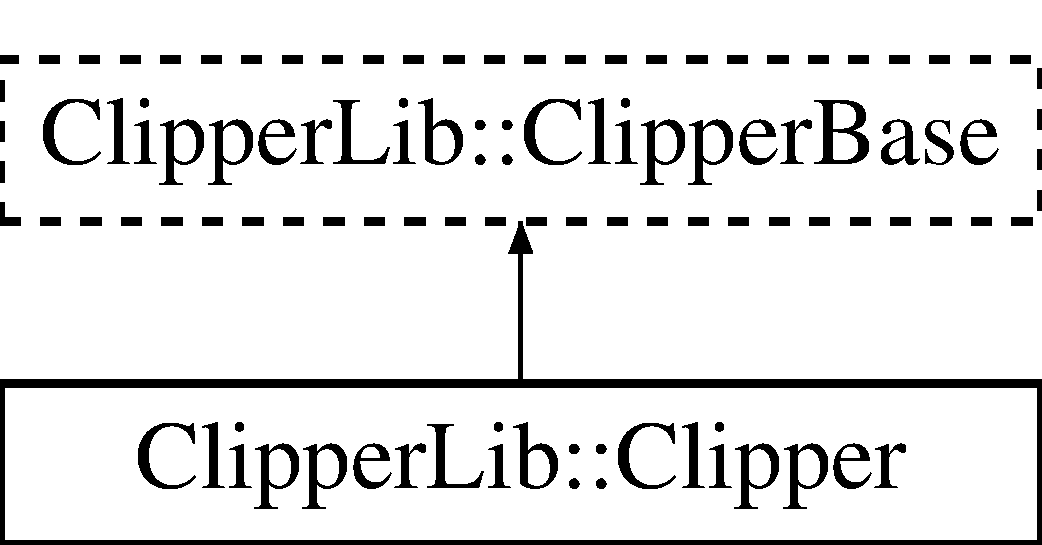
\includegraphics[height=2.000000cm]{classClipperLib_1_1Clipper}
\end{center}
\end{figure}
\subsection*{Public Member Functions}
\begin{DoxyCompactItemize}
\item 
\hypertarget{classClipperLib_1_1Clipper_a674d5d300c73a4da99bc36a7ecde0618}{bool {\bfseries Execute} (Clip\-Type clip\-Type, Polygons \&solution, Poly\-Fill\-Type subj\-Fill\-Type=pft\-Even\-Odd, Poly\-Fill\-Type clip\-Fill\-Type=pft\-Even\-Odd)}\label{classClipperLib_1_1Clipper_a674d5d300c73a4da99bc36a7ecde0618}

\item 
\hypertarget{classClipperLib_1_1Clipper_aceb19a1e5a5c9e31067f4d1177793403}{bool {\bfseries Execute} (Clip\-Type clip\-Type, \hyperlink{classClipperLib_1_1PolyTree}{Poly\-Tree} \&polytree, Poly\-Fill\-Type subj\-Fill\-Type=pft\-Even\-Odd, Poly\-Fill\-Type clip\-Fill\-Type=pft\-Even\-Odd)}\label{classClipperLib_1_1Clipper_aceb19a1e5a5c9e31067f4d1177793403}

\item 
\hypertarget{classClipperLib_1_1Clipper_a4f4576bad48bce34a36e6806623abd7a}{void {\bfseries Clear} ()}\label{classClipperLib_1_1Clipper_a4f4576bad48bce34a36e6806623abd7a}

\item 
\hypertarget{classClipperLib_1_1Clipper_ad556ba9961f498de02d55dc95bc5a889}{bool {\bfseries Reverse\-Solution} ()}\label{classClipperLib_1_1Clipper_ad556ba9961f498de02d55dc95bc5a889}

\item 
\hypertarget{classClipperLib_1_1Clipper_a44afc0c82a1d2607829b5fd21f7644ef}{void {\bfseries Reverse\-Solution} (bool value)}\label{classClipperLib_1_1Clipper_a44afc0c82a1d2607829b5fd21f7644ef}

\end{DoxyCompactItemize}
\subsection*{Protected Member Functions}
\begin{DoxyCompactItemize}
\item 
\hypertarget{classClipperLib_1_1Clipper_a14c704b062e8a079e34a8ce40838861e}{void {\bfseries Reset} ()}\label{classClipperLib_1_1Clipper_a14c704b062e8a079e34a8ce40838861e}

\item 
\hypertarget{classClipperLib_1_1Clipper_a3e8757e5f8a6ffcb7fd0f9630fde02d3}{virtual bool {\bfseries Execute\-Internal} ()}\label{classClipperLib_1_1Clipper_a3e8757e5f8a6ffcb7fd0f9630fde02d3}

\end{DoxyCompactItemize}
\subsection*{Additional Inherited Members}


The documentation for this class was generated from the following files\-:\begin{DoxyCompactItemize}
\item 
model/clipper/clipper.\-hpp\item 
model/clipper/clipper.\-cpp\end{DoxyCompactItemize}

\hypertarget{classClipperLib_1_1ClipperBase}{\section{Clipper\-Lib\-:\-:Clipper\-Base Class Reference}
\label{classClipperLib_1_1ClipperBase}\index{Clipper\-Lib\-::\-Clipper\-Base@{Clipper\-Lib\-::\-Clipper\-Base}}
}
Inheritance diagram for Clipper\-Lib\-:\-:Clipper\-Base\-:\begin{figure}[H]
\begin{center}
\leavevmode
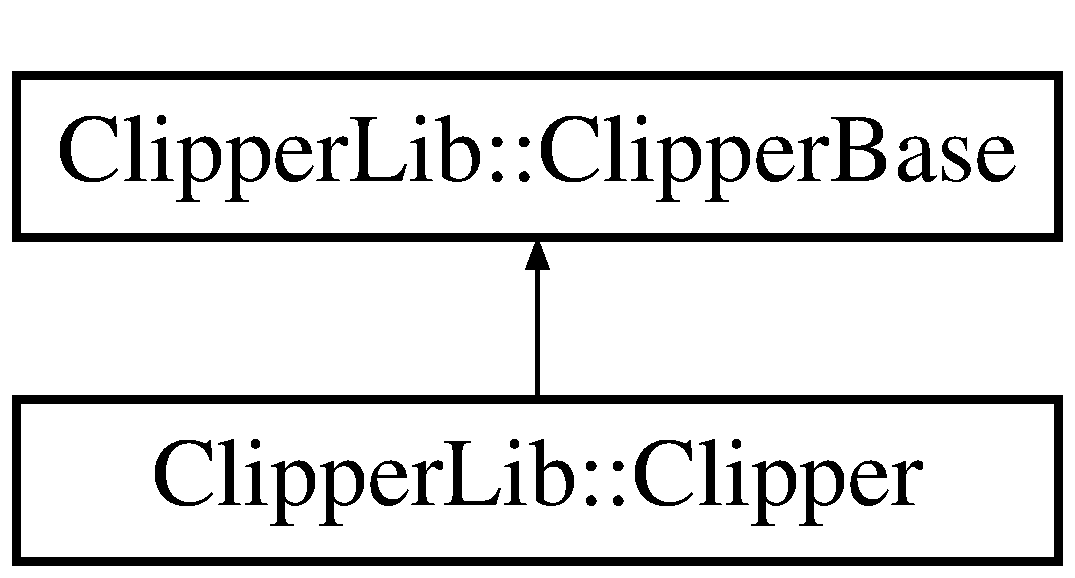
\includegraphics[height=2.000000cm]{classClipperLib_1_1ClipperBase}
\end{center}
\end{figure}
\subsection*{Public Member Functions}
\begin{DoxyCompactItemize}
\item 
\hypertarget{classClipperLib_1_1ClipperBase_a62f7b073052eed2d0ee9af69a237badd}{bool {\bfseries Add\-Polygon} (const \hyperlink{classPolygon}{Polygon} \&pg, Poly\-Type poly\-Type)}\label{classClipperLib_1_1ClipperBase_a62f7b073052eed2d0ee9af69a237badd}

\item 
\hypertarget{classClipperLib_1_1ClipperBase_a5cdf386f8ba72b196dec6ad0a8607bbf}{bool {\bfseries Add\-Polygons} (const Polygons \&ppg, Poly\-Type poly\-Type)}\label{classClipperLib_1_1ClipperBase_a5cdf386f8ba72b196dec6ad0a8607bbf}

\item 
\hypertarget{classClipperLib_1_1ClipperBase_a5690952fe8c2cb047025566405827821}{virtual void {\bfseries Clear} ()}\label{classClipperLib_1_1ClipperBase_a5690952fe8c2cb047025566405827821}

\item 
\hypertarget{classClipperLib_1_1ClipperBase_a5590a5454248ac3f6beeba7f9690f62e}{\hyperlink{structClipperLib_1_1IntRect}{Int\-Rect} {\bfseries Get\-Bounds} ()}\label{classClipperLib_1_1ClipperBase_a5590a5454248ac3f6beeba7f9690f62e}

\end{DoxyCompactItemize}
\subsection*{Protected Member Functions}
\begin{DoxyCompactItemize}
\item 
\hypertarget{classClipperLib_1_1ClipperBase_a311dbbec1454ab7965e363a0359f5ee4}{void {\bfseries Dispose\-Local\-Minima\-List} ()}\label{classClipperLib_1_1ClipperBase_a311dbbec1454ab7965e363a0359f5ee4}

\item 
\hypertarget{classClipperLib_1_1ClipperBase_a2e70686545484c6767dead34d9673ebe}{\hyperlink{structClipperLib_1_1TEdge}{T\-Edge} $\ast$ {\bfseries Add\-Bounds\-To\-L\-M\-L} (\hyperlink{structClipperLib_1_1TEdge}{T\-Edge} $\ast$e)}\label{classClipperLib_1_1ClipperBase_a2e70686545484c6767dead34d9673ebe}

\item 
\hypertarget{classClipperLib_1_1ClipperBase_a9554e9f2273c39e0f5f07d3cd73533e6}{void {\bfseries Pop\-Local\-Minima} ()}\label{classClipperLib_1_1ClipperBase_a9554e9f2273c39e0f5f07d3cd73533e6}

\item 
\hypertarget{classClipperLib_1_1ClipperBase_a125febb065f23fc55dafffe8d185b642}{virtual void {\bfseries Reset} ()}\label{classClipperLib_1_1ClipperBase_a125febb065f23fc55dafffe8d185b642}

\item 
\hypertarget{classClipperLib_1_1ClipperBase_aa62506f423172bccd6de8a645cc29cff}{void {\bfseries Insert\-Local\-Minima} (\hyperlink{structClipperLib_1_1LocalMinima}{Local\-Minima} $\ast$new\-Lm)}\label{classClipperLib_1_1ClipperBase_aa62506f423172bccd6de8a645cc29cff}

\end{DoxyCompactItemize}
\subsection*{Protected Attributes}
\begin{DoxyCompactItemize}
\item 
\hypertarget{classClipperLib_1_1ClipperBase_a4e3039382d3c8ec6f9ab434021be8d43}{\hyperlink{structClipperLib_1_1LocalMinima}{Local\-Minima} $\ast$ {\bfseries m\-\_\-\-Current\-L\-M}}\label{classClipperLib_1_1ClipperBase_a4e3039382d3c8ec6f9ab434021be8d43}

\item 
\hypertarget{classClipperLib_1_1ClipperBase_a74df45b228436fa0243b53cc00192a5f}{\hyperlink{structClipperLib_1_1LocalMinima}{Local\-Minima} $\ast$ {\bfseries m\-\_\-\-Minima\-List}}\label{classClipperLib_1_1ClipperBase_a74df45b228436fa0243b53cc00192a5f}

\item 
\hypertarget{classClipperLib_1_1ClipperBase_aea11d183617adc12d7ba2b84533f7f45}{bool {\bfseries m\-\_\-\-Use\-Full\-Range}}\label{classClipperLib_1_1ClipperBase_aea11d183617adc12d7ba2b84533f7f45}

\item 
\hypertarget{classClipperLib_1_1ClipperBase_a8bfc007c0c0afd4e9d252dac0ef5daa0}{Edge\-List {\bfseries m\-\_\-edges}}\label{classClipperLib_1_1ClipperBase_a8bfc007c0c0afd4e9d252dac0ef5daa0}

\end{DoxyCompactItemize}


The documentation for this class was generated from the following files\-:\begin{DoxyCompactItemize}
\item 
model/clipper/clipper.\-hpp\item 
model/clipper/clipper.\-cpp\end{DoxyCompactItemize}

\hypertarget{classClipperLib_1_1clipperException}{\section{Clipper\-Lib\-:\-:clipper\-Exception Class Reference}
\label{classClipperLib_1_1clipperException}\index{Clipper\-Lib\-::clipper\-Exception@{Clipper\-Lib\-::clipper\-Exception}}
}
Inheritance diagram for Clipper\-Lib\-:\-:clipper\-Exception\-:\begin{figure}[H]
\begin{center}
\leavevmode
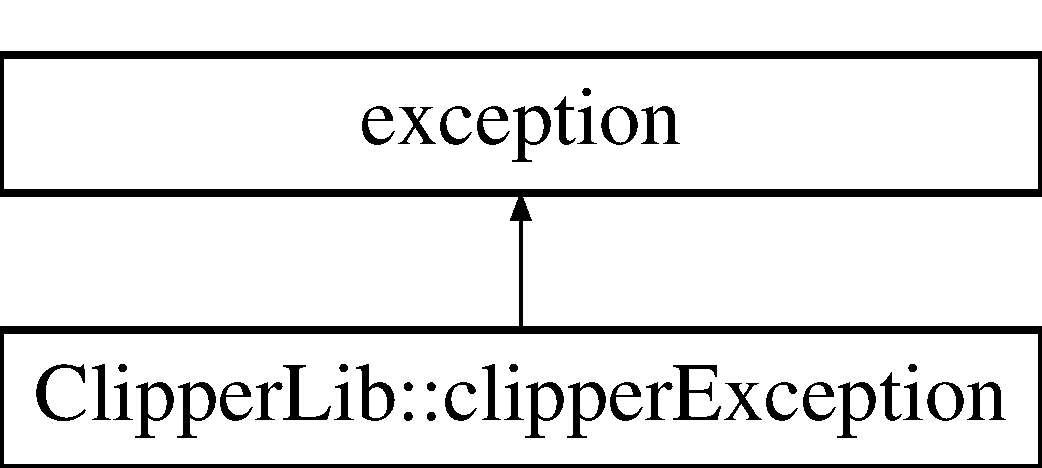
\includegraphics[height=2.000000cm]{classClipperLib_1_1clipperException}
\end{center}
\end{figure}
\subsection*{Public Member Functions}
\begin{DoxyCompactItemize}
\item 
\hypertarget{classClipperLib_1_1clipperException_a7d44b32d06cd870500355667f6e0d6ed}{{\bfseries clipper\-Exception} (const char $\ast$description)}\label{classClipperLib_1_1clipperException_a7d44b32d06cd870500355667f6e0d6ed}

\item 
\hypertarget{classClipperLib_1_1clipperException_a7bd8c881bda597f839670dde97fe04d4}{virtual const char $\ast$ {\bfseries what} () const   throw ()}\label{classClipperLib_1_1clipperException_a7bd8c881bda597f839670dde97fe04d4}

\end{DoxyCompactItemize}


The documentation for this class was generated from the following file\-:\begin{DoxyCompactItemize}
\item 
model/clipper/clipper.\-hpp\end{DoxyCompactItemize}

\hypertarget{structClipperLib_1_1DoublePoint}{\section{Clipper\-Lib\-:\-:Double\-Point Struct Reference}
\label{structClipperLib_1_1DoublePoint}\index{Clipper\-Lib\-::\-Double\-Point@{Clipper\-Lib\-::\-Double\-Point}}
}
\subsection*{Public Member Functions}
\begin{DoxyCompactItemize}
\item 
\hypertarget{structClipperLib_1_1DoublePoint_a3ccbea6aaf488e0a2d8ac499d2676093}{{\bfseries Double\-Point} (double x=0, double y=0)}\label{structClipperLib_1_1DoublePoint_a3ccbea6aaf488e0a2d8ac499d2676093}

\end{DoxyCompactItemize}
\subsection*{Public Attributes}
\begin{DoxyCompactItemize}
\item 
\hypertarget{structClipperLib_1_1DoublePoint_a675837cc05f20447313789b82d84ad31}{double {\bfseries X}}\label{structClipperLib_1_1DoublePoint_a675837cc05f20447313789b82d84ad31}

\item 
\hypertarget{structClipperLib_1_1DoublePoint_a49774a93540882d88448badf37034454}{double {\bfseries Y}}\label{structClipperLib_1_1DoublePoint_a49774a93540882d88448badf37034454}

\end{DoxyCompactItemize}


The documentation for this struct was generated from the following file\-:\begin{DoxyCompactItemize}
\item 
model/clipper/clipper.\-cpp\end{DoxyCompactItemize}

\input{structmodel_1_1DtrmEvent}
\input{classmodel_1_1Facade}
\input{classmodel_1_1Formula}
\input{structFormula}
\input{classmodel_1_1GeometryHelper}
\hypertarget{classGUIController}{\section{G\-U\-I\-Controller Class Reference}
\label{classGUIController}\index{G\-U\-I\-Controller@{G\-U\-I\-Controller}}
}
Inheritance diagram for G\-U\-I\-Controller\-:\begin{figure}[H]
\begin{center}
\leavevmode
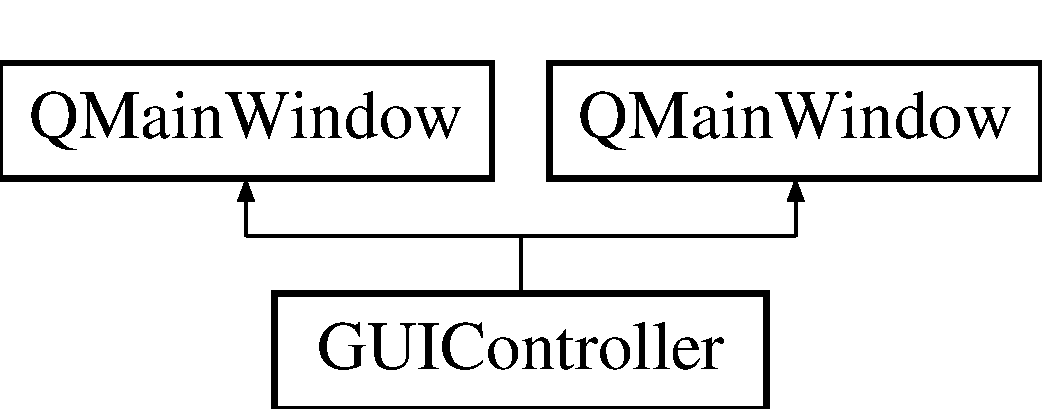
\includegraphics[height=2.000000cm]{classGUIController}
\end{center}
\end{figure}
\subsection*{Public Member Functions}
\begin{DoxyCompactItemize}
\item 
\hyperlink{classGUIController_a3f85fdeac642a3c52c0f0b586462eb8a}{G\-U\-I\-Controller} (Q\-Widget $\ast$parent=0)
\begin{DoxyCompactList}\small\item\em \hyperlink{classGUIController}{G\-U\-I\-Controller} is the constructor of the main window. The main window constructs all the elements via the ui file. The title of the main window is set to the tool name. The position of the main window is adjusted to the center. The default empty files are initiated. \end{DoxyCompactList}\item 
\hypertarget{classGUIController_acf3b4a6d7ab7be45f20ab41831644444}{\hyperlink{classGUIController_acf3b4a6d7ab7be45f20ab41831644444}{$\sim$\-G\-U\-I\-Controller} ()}\label{classGUIController_acf3b4a6d7ab7be45f20ab41831644444}

\begin{DoxyCompactList}\small\item\em The destroyer that frees the memory The ui is deleted and the memory is freed. \end{DoxyCompactList}\item 
void \hyperlink{classGUIController_a3e67be4bfe8c3ebdf943540e1b06949b}{add\-Text} (std\-::string str)
\begin{DoxyCompactList}\small\item\em Add a normal text to the build-\/in terminal. \end{DoxyCompactList}\item 
void \hyperlink{classGUIController_ac57ebab895a0f83ca9c09fd60d835585}{add\-Success} (std\-::string str)
\begin{DoxyCompactList}\small\item\em Add an success text to the build-\/in terminal. \end{DoxyCompactList}\item 
void \hyperlink{classGUIController_a5ea3697ae0408cb521e82a0b315d2661}{add\-Warning} (std\-::string str)
\begin{DoxyCompactList}\small\item\em Add a warning text to the build-\/in terminal. \end{DoxyCompactList}\item 
void \hyperlink{classGUIController_a8b5677300791307f8597dc427772ad11}{add\-Error} (std\-::string str)
\begin{DoxyCompactList}\small\item\em Add an error text to the build-\/in terminal. \end{DoxyCompactList}\item 
void \hyperlink{classGUIController_aff7752195a9d8c86d326f212ccda1e7b}{set\-Text} (std\-::string str)
\begin{DoxyCompactList}\small\item\em Set the text in the build-\/in terminal. \end{DoxyCompactList}\item 
std\-::string \hyperlink{classGUIController_a494d1c2423ce3e7d44633edc50269803}{get\-Text} ()
\begin{DoxyCompactList}\small\item\em Give the current text of the build-\/in terminal. \end{DoxyCompactList}\item 
\hypertarget{classGUIController_a3f85fdeac642a3c52c0f0b586462eb8a}{{\bfseries G\-U\-I\-Controller} (Q\-Widget $\ast$parent=0)}\label{classGUIController_a3f85fdeac642a3c52c0f0b586462eb8a}

\end{DoxyCompactItemize}
\subsection*{Protected Member Functions}
\begin{DoxyCompactItemize}
\item 
void \hyperlink{classGUIController_ae675a28ff6534f3443910cdf1c8d6603}{close\-Event} (Q\-Close\-Event $\ast$event)
\begin{DoxyCompactList}\small\item\em Check if the files are saved when the window is closed. \end{DoxyCompactList}\item 
\hypertarget{classGUIController_ae675a28ff6534f3443910cdf1c8d6603}{void {\bfseries close\-Event} (Q\-Close\-Event $\ast$event)}\label{classGUIController_ae675a28ff6534f3443910cdf1c8d6603}

\end{DoxyCompactItemize}


\subsection{Constructor \& Destructor Documentation}
\hypertarget{classGUIController_a3f85fdeac642a3c52c0f0b586462eb8a}{\index{G\-U\-I\-Controller@{G\-U\-I\-Controller}!G\-U\-I\-Controller@{G\-U\-I\-Controller}}
\index{G\-U\-I\-Controller@{G\-U\-I\-Controller}!GUIController@{G\-U\-I\-Controller}}
\subsubsection[{G\-U\-I\-Controller}]{\setlength{\rightskip}{0pt plus 5cm}G\-U\-I\-Controller\-::\-G\-U\-I\-Controller (
\begin{DoxyParamCaption}
\item[{Q\-Widget $\ast$}]{parent = {\ttfamily 0}}
\end{DoxyParamCaption}
)\hspace{0.3cm}{\ttfamily [explicit]}}}\label{classGUIController_a3f85fdeac642a3c52c0f0b586462eb8a}


\hyperlink{classGUIController}{G\-U\-I\-Controller} is the constructor of the main window. The main window constructs all the elements via the ui file. The title of the main window is set to the tool name. The position of the main window is adjusted to the center. The default empty files are initiated. 

F\-S\-T\-Gui\-::\-F\-S\-T\-Gui is the constructor of the main window. The main window constructs all the elements via the ui file. The title of the main window is set to the tool name. The position of the main window is adjusted to the center. The default empty files are initiated.


\begin{DoxyParams}{Parameters}
{\em parent} & the parent Q\-Widget \\
\hline
\end{DoxyParams}


\subsection{Member Function Documentation}
\hypertarget{classGUIController_a8b5677300791307f8597dc427772ad11}{\index{G\-U\-I\-Controller@{G\-U\-I\-Controller}!add\-Error@{add\-Error}}
\index{add\-Error@{add\-Error}!GUIController@{G\-U\-I\-Controller}}
\subsubsection[{add\-Error}]{\setlength{\rightskip}{0pt plus 5cm}void G\-U\-I\-Controller\-::add\-Error (
\begin{DoxyParamCaption}
\item[{std\-::string}]{str}
\end{DoxyParamCaption}
)\hspace{0.3cm}{\ttfamily [virtual]}}}\label{classGUIController_a8b5677300791307f8597dc427772ad11}


Add an error text to the build-\/in terminal. 

\hyperlink{classGUIController_a3e67be4bfe8c3ebdf943540e1b06949b}{G\-U\-I\-Controller\-::add\-Text} Add an error text to the build-\/in terminal.


\begin{DoxyParams}{Parameters}
{\em str} & String containing the text to be added. \\
\hline
\end{DoxyParams}


Implements \hyperlink{classmodel_1_1Logger}{model\-::\-Logger}.

\hypertarget{classGUIController_ac57ebab895a0f83ca9c09fd60d835585}{\index{G\-U\-I\-Controller@{G\-U\-I\-Controller}!add\-Success@{add\-Success}}
\index{add\-Success@{add\-Success}!GUIController@{G\-U\-I\-Controller}}
\subsubsection[{add\-Success}]{\setlength{\rightskip}{0pt plus 5cm}void G\-U\-I\-Controller\-::add\-Success (
\begin{DoxyParamCaption}
\item[{std\-::string}]{str}
\end{DoxyParamCaption}
)\hspace{0.3cm}{\ttfamily [virtual]}}}\label{classGUIController_ac57ebab895a0f83ca9c09fd60d835585}


Add an success text to the build-\/in terminal. 

\hyperlink{classGUIController_a3e67be4bfe8c3ebdf943540e1b06949b}{G\-U\-I\-Controller\-::add\-Text} Add an information text to the build-\/in terminal.


\begin{DoxyParams}{Parameters}
{\em str} & String containing the text to be added. \\
\hline
\end{DoxyParams}


Implements \hyperlink{classmodel_1_1Logger}{model\-::\-Logger}.

\hypertarget{classGUIController_a3e67be4bfe8c3ebdf943540e1b06949b}{\index{G\-U\-I\-Controller@{G\-U\-I\-Controller}!add\-Text@{add\-Text}}
\index{add\-Text@{add\-Text}!GUIController@{G\-U\-I\-Controller}}
\subsubsection[{add\-Text}]{\setlength{\rightskip}{0pt plus 5cm}void G\-U\-I\-Controller\-::add\-Text (
\begin{DoxyParamCaption}
\item[{std\-::string}]{str}
\end{DoxyParamCaption}
)\hspace{0.3cm}{\ttfamily [virtual]}}}\label{classGUIController_a3e67be4bfe8c3ebdf943540e1b06949b}


Add a normal text to the build-\/in terminal. 

\hyperlink{classGUIController_a3e67be4bfe8c3ebdf943540e1b06949b}{G\-U\-I\-Controller\-::add\-Text} Add a normal text to the build-\/in terminal.


\begin{DoxyParams}{Parameters}
{\em str} & String containing the text to be added. \\
\hline
\end{DoxyParams}


Implements \hyperlink{classmodel_1_1Logger}{model\-::\-Logger}.

\hypertarget{classGUIController_a5ea3697ae0408cb521e82a0b315d2661}{\index{G\-U\-I\-Controller@{G\-U\-I\-Controller}!add\-Warning@{add\-Warning}}
\index{add\-Warning@{add\-Warning}!GUIController@{G\-U\-I\-Controller}}
\subsubsection[{add\-Warning}]{\setlength{\rightskip}{0pt plus 5cm}void G\-U\-I\-Controller\-::add\-Warning (
\begin{DoxyParamCaption}
\item[{std\-::string}]{str}
\end{DoxyParamCaption}
)\hspace{0.3cm}{\ttfamily [virtual]}}}\label{classGUIController_a5ea3697ae0408cb521e82a0b315d2661}


Add a warning text to the build-\/in terminal. 

\hyperlink{classGUIController_a3e67be4bfe8c3ebdf943540e1b06949b}{G\-U\-I\-Controller\-::add\-Text} Add a warning text to the build-\/in terminal.


\begin{DoxyParams}{Parameters}
{\em str} & String containing the text to be added. \\
\hline
\end{DoxyParams}


Implements \hyperlink{classmodel_1_1Logger}{model\-::\-Logger}.

\hypertarget{classGUIController_ae675a28ff6534f3443910cdf1c8d6603}{\index{G\-U\-I\-Controller@{G\-U\-I\-Controller}!close\-Event@{close\-Event}}
\index{close\-Event@{close\-Event}!GUIController@{G\-U\-I\-Controller}}
\subsubsection[{close\-Event}]{\setlength{\rightskip}{0pt plus 5cm}void G\-U\-I\-Controller\-::close\-Event (
\begin{DoxyParamCaption}
\item[{Q\-Close\-Event $\ast$}]{event}
\end{DoxyParamCaption}
)\hspace{0.3cm}{\ttfamily [protected]}}}\label{classGUIController_ae675a28ff6534f3443910cdf1c8d6603}


Check if the files are saved when the window is closed. 


\begin{DoxyParams}[1]{Parameters}
\mbox{\tt out}  & {\em event} & The closing event. \\
\hline
\end{DoxyParams}
\hypertarget{classGUIController_a494d1c2423ce3e7d44633edc50269803}{\index{G\-U\-I\-Controller@{G\-U\-I\-Controller}!get\-Text@{get\-Text}}
\index{get\-Text@{get\-Text}!GUIController@{G\-U\-I\-Controller}}
\subsubsection[{get\-Text}]{\setlength{\rightskip}{0pt plus 5cm}std\-::string G\-U\-I\-Controller\-::get\-Text (
\begin{DoxyParamCaption}
{}
\end{DoxyParamCaption}
)\hspace{0.3cm}{\ttfamily [virtual]}}}\label{classGUIController_a494d1c2423ce3e7d44633edc50269803}


Give the current text of the build-\/in terminal. 

\begin{DoxyReturn}{Returns}
Gives a Q\-String text of the build-\/in terminal. 
\end{DoxyReturn}


Implements \hyperlink{classmodel_1_1Logger}{model\-::\-Logger}.

\hypertarget{classGUIController_aff7752195a9d8c86d326f212ccda1e7b}{\index{G\-U\-I\-Controller@{G\-U\-I\-Controller}!set\-Text@{set\-Text}}
\index{set\-Text@{set\-Text}!GUIController@{G\-U\-I\-Controller}}
\subsubsection[{set\-Text}]{\setlength{\rightskip}{0pt plus 5cm}void G\-U\-I\-Controller\-::set\-Text (
\begin{DoxyParamCaption}
\item[{std\-::string}]{str}
\end{DoxyParamCaption}
)\hspace{0.3cm}{\ttfamily [virtual]}}}\label{classGUIController_aff7752195a9d8c86d326f212ccda1e7b}


Set the text in the build-\/in terminal. 


\begin{DoxyParams}{Parameters}
{\em str} & String containing the text to be set. \\
\hline
\end{DoxyParams}


Implements \hyperlink{classmodel_1_1Logger}{model\-::\-Logger}.



The documentation for this class was generated from the following files\-:\begin{DoxyCompactItemize}
\item 
controller/G\-U\-I\-Controller.\-h\item 
view/G\-U\-I\-Controller.\-h\item 
controller/G\-U\-I\-Controller.\-cpp\item 
view/G\-U\-I\-Controller.\-cpp\end{DoxyCompactItemize}

\hypertarget{structClipperLib_1_1HorzJoinRec}{\section{Clipper\-Lib\-:\-:Horz\-Join\-Rec Struct Reference}
\label{structClipperLib_1_1HorzJoinRec}\index{Clipper\-Lib\-::\-Horz\-Join\-Rec@{Clipper\-Lib\-::\-Horz\-Join\-Rec}}
}
\subsection*{Public Attributes}
\begin{DoxyCompactItemize}
\item 
\hypertarget{structClipperLib_1_1HorzJoinRec_a610c6cf1e5edfc418da0965c3f68a8b8}{\hyperlink{structClipperLib_1_1TEdge}{T\-Edge} $\ast$ {\bfseries edge}}\label{structClipperLib_1_1HorzJoinRec_a610c6cf1e5edfc418da0965c3f68a8b8}

\item 
\hypertarget{structClipperLib_1_1HorzJoinRec_a58dada80e24143e14c71458340099b14}{int {\bfseries saved\-Idx}}\label{structClipperLib_1_1HorzJoinRec_a58dada80e24143e14c71458340099b14}

\end{DoxyCompactItemize}


The documentation for this struct was generated from the following file\-:\begin{DoxyCompactItemize}
\item 
model/clipper/clipper.\-hpp\end{DoxyCompactItemize}

\hypertarget{classClipperLib_1_1Int128}{\section{Clipper\-Lib\-:\-:Int128 Class Reference}
\label{classClipperLib_1_1Int128}\index{Clipper\-Lib\-::\-Int128@{Clipper\-Lib\-::\-Int128}}
}
\subsection*{Public Member Functions}
\begin{DoxyCompactItemize}
\item 
\hypertarget{classClipperLib_1_1Int128_acb7953a56e0ddb6d3245268e457f9e37}{{\bfseries Int128} (long64 \-\_\-lo=0)}\label{classClipperLib_1_1Int128_acb7953a56e0ddb6d3245268e457f9e37}

\item 
\hypertarget{classClipperLib_1_1Int128_ad113c3dc3bd371984b05fddb1fe527e2}{{\bfseries Int128} (const \hyperlink{classClipperLib_1_1Int128}{Int128} \&val)}\label{classClipperLib_1_1Int128_ad113c3dc3bd371984b05fddb1fe527e2}

\item 
\hypertarget{classClipperLib_1_1Int128_ac23a17a6a5ea143f0297b7ba0dd1830e}{{\bfseries Int128} (const long64 \&\-\_\-hi, const ulong64 \&\-\_\-lo)}\label{classClipperLib_1_1Int128_ac23a17a6a5ea143f0297b7ba0dd1830e}

\item 
\hypertarget{classClipperLib_1_1Int128_a51ef81c338951a30c55315d43bdf2690}{long64 {\bfseries operator=} (const long64 \&val)}\label{classClipperLib_1_1Int128_a51ef81c338951a30c55315d43bdf2690}

\item 
\hypertarget{classClipperLib_1_1Int128_a9a4597562962e318616a463350c68896}{bool {\bfseries operator==} (const \hyperlink{classClipperLib_1_1Int128}{Int128} \&val) const }\label{classClipperLib_1_1Int128_a9a4597562962e318616a463350c68896}

\item 
\hypertarget{classClipperLib_1_1Int128_a4b79b3e28a4012f87d03fc02969796f9}{bool {\bfseries operator!=} (const \hyperlink{classClipperLib_1_1Int128}{Int128} \&val) const }\label{classClipperLib_1_1Int128_a4b79b3e28a4012f87d03fc02969796f9}

\item 
\hypertarget{classClipperLib_1_1Int128_af34c23b86068c7f065a76dbc1d192269}{bool {\bfseries operator$>$} (const \hyperlink{classClipperLib_1_1Int128}{Int128} \&val) const }\label{classClipperLib_1_1Int128_af34c23b86068c7f065a76dbc1d192269}

\item 
\hypertarget{classClipperLib_1_1Int128_a1f875f6f5357bdb031dc4ef0d058268d}{bool {\bfseries operator$<$} (const \hyperlink{classClipperLib_1_1Int128}{Int128} \&val) const }\label{classClipperLib_1_1Int128_a1f875f6f5357bdb031dc4ef0d058268d}

\item 
\hypertarget{classClipperLib_1_1Int128_a1e8869c867b94465a5e4b54de49d6c11}{bool {\bfseries operator$>$=} (const \hyperlink{classClipperLib_1_1Int128}{Int128} \&val) const }\label{classClipperLib_1_1Int128_a1e8869c867b94465a5e4b54de49d6c11}

\item 
\hypertarget{classClipperLib_1_1Int128_a2c45d01fdcbf15015aff79d491c97416}{bool {\bfseries operator$<$=} (const \hyperlink{classClipperLib_1_1Int128}{Int128} \&val) const }\label{classClipperLib_1_1Int128_a2c45d01fdcbf15015aff79d491c97416}

\item 
\hypertarget{classClipperLib_1_1Int128_ad48a700134ab5c4e08bd53966b731950}{\hyperlink{classClipperLib_1_1Int128}{Int128} \& {\bfseries operator+=} (const \hyperlink{classClipperLib_1_1Int128}{Int128} \&rhs)}\label{classClipperLib_1_1Int128_ad48a700134ab5c4e08bd53966b731950}

\item 
\hypertarget{classClipperLib_1_1Int128_acb2d49860fb6ddf5b598ac6e15ac9521}{\hyperlink{classClipperLib_1_1Int128}{Int128} {\bfseries operator+} (const \hyperlink{classClipperLib_1_1Int128}{Int128} \&rhs) const }\label{classClipperLib_1_1Int128_acb2d49860fb6ddf5b598ac6e15ac9521}

\item 
\hypertarget{classClipperLib_1_1Int128_a7b35c74c15392ae8d48c031f750c1b28}{\hyperlink{classClipperLib_1_1Int128}{Int128} \& {\bfseries operator-\/=} (const \hyperlink{classClipperLib_1_1Int128}{Int128} \&rhs)}\label{classClipperLib_1_1Int128_a7b35c74c15392ae8d48c031f750c1b28}

\item 
\hypertarget{classClipperLib_1_1Int128_a9ab61c357c61a3f3ad5fc628e36879e2}{\hyperlink{classClipperLib_1_1Int128}{Int128} {\bfseries operator-\/} (const \hyperlink{classClipperLib_1_1Int128}{Int128} \&rhs) const }\label{classClipperLib_1_1Int128_a9ab61c357c61a3f3ad5fc628e36879e2}

\item 
\hypertarget{classClipperLib_1_1Int128_af1c84872b2d290230a0f68fb97013d4d}{\hyperlink{classClipperLib_1_1Int128}{Int128} {\bfseries operator-\/} () const }\label{classClipperLib_1_1Int128_af1c84872b2d290230a0f68fb97013d4d}

\item 
\hypertarget{classClipperLib_1_1Int128_a91718f7da0f2442e03e69b019f21dd7d}{\hyperlink{classClipperLib_1_1Int128}{Int128} {\bfseries operator/} (const \hyperlink{classClipperLib_1_1Int128}{Int128} \&rhs) const }\label{classClipperLib_1_1Int128_a91718f7da0f2442e03e69b019f21dd7d}

\item 
\hypertarget{classClipperLib_1_1Int128_a6629ebee1d059ea486c789eaa24fb994}{double {\bfseries As\-Double} () const }\label{classClipperLib_1_1Int128_a6629ebee1d059ea486c789eaa24fb994}

\end{DoxyCompactItemize}
\subsection*{Public Attributes}
\begin{DoxyCompactItemize}
\item 
\hypertarget{classClipperLib_1_1Int128_a991b9da6e53c777a94fca640e505b258}{ulong64 {\bfseries lo}}\label{classClipperLib_1_1Int128_a991b9da6e53c777a94fca640e505b258}

\item 
\hypertarget{classClipperLib_1_1Int128_a167643d0860a14fb563e055511e15e14}{long64 {\bfseries hi}}\label{classClipperLib_1_1Int128_a167643d0860a14fb563e055511e15e14}

\end{DoxyCompactItemize}


The documentation for this class was generated from the following file\-:\begin{DoxyCompactItemize}
\item 
model/clipper/clipper.\-cpp\end{DoxyCompactItemize}

\hypertarget{structClipperLib_1_1IntersectNode}{\section{Clipper\-Lib\-:\-:Intersect\-Node Struct Reference}
\label{structClipperLib_1_1IntersectNode}\index{Clipper\-Lib\-::\-Intersect\-Node@{Clipper\-Lib\-::\-Intersect\-Node}}
}
\subsection*{Public Attributes}
\begin{DoxyCompactItemize}
\item 
\hypertarget{structClipperLib_1_1IntersectNode_a9ca23b5341d4609ecb24ad7ac5eb6da4}{\hyperlink{structClipperLib_1_1TEdge}{T\-Edge} $\ast$ {\bfseries edge1}}\label{structClipperLib_1_1IntersectNode_a9ca23b5341d4609ecb24ad7ac5eb6da4}

\item 
\hypertarget{structClipperLib_1_1IntersectNode_ac32451de72e8e929bbb9704b8d330317}{\hyperlink{structClipperLib_1_1TEdge}{T\-Edge} $\ast$ {\bfseries edge2}}\label{structClipperLib_1_1IntersectNode_ac32451de72e8e929bbb9704b8d330317}

\item 
\hypertarget{structClipperLib_1_1IntersectNode_af24af801ac1e74f9200908dcad88cc30}{\hyperlink{structClipperLib_1_1IntPoint}{Int\-Point} {\bfseries pt}}\label{structClipperLib_1_1IntersectNode_af24af801ac1e74f9200908dcad88cc30}

\item 
\hypertarget{structClipperLib_1_1IntersectNode_a6534367f8cc07404d5f19230166f8c78}{\hyperlink{structClipperLib_1_1IntersectNode}{Intersect\-Node} $\ast$ {\bfseries next}}\label{structClipperLib_1_1IntersectNode_a6534367f8cc07404d5f19230166f8c78}

\end{DoxyCompactItemize}


The documentation for this struct was generated from the following file\-:\begin{DoxyCompactItemize}
\item 
model/clipper/clipper.\-hpp\end{DoxyCompactItemize}

\input{structInterval}
\input{classmodel_1_1Interval}
\input{classmodel_1_1IntervalSet}
\hypertarget{structClipperLib_1_1IntPoint}{\section{Clipper\-Lib\-:\-:Int\-Point Struct Reference}
\label{structClipperLib_1_1IntPoint}\index{Clipper\-Lib\-::\-Int\-Point@{Clipper\-Lib\-::\-Int\-Point}}
}
\subsection*{Public Member Functions}
\begin{DoxyCompactItemize}
\item 
\hypertarget{structClipperLib_1_1IntPoint_a455b8d5c7f6d4c8e5adebcac8fa11e71}{{\bfseries Int\-Point} (long64 x=0, long64 y=0)}\label{structClipperLib_1_1IntPoint_a455b8d5c7f6d4c8e5adebcac8fa11e71}

\end{DoxyCompactItemize}
\subsection*{Public Attributes}
\begin{DoxyCompactItemize}
\item 
\hypertarget{structClipperLib_1_1IntPoint_af47546895f6b0403abf4701cb00bd6fa}{long64 {\bfseries X}}\label{structClipperLib_1_1IntPoint_af47546895f6b0403abf4701cb00bd6fa}

\item 
\hypertarget{structClipperLib_1_1IntPoint_a24a7d31ef4e1a5d8a70e7e29f5429011}{long64 {\bfseries Y}}\label{structClipperLib_1_1IntPoint_a24a7d31ef4e1a5d8a70e7e29f5429011}

\end{DoxyCompactItemize}
\subsection*{Friends}
\begin{DoxyCompactItemize}
\item 
\hypertarget{structClipperLib_1_1IntPoint_a9d7a086edc8217df9f23c9c1635e2fd9}{std\-::ostream \& {\bfseries operator$<$$<$} (std\-::ostream \&s, \hyperlink{structClipperLib_1_1IntPoint}{Int\-Point} \&p)}\label{structClipperLib_1_1IntPoint_a9d7a086edc8217df9f23c9c1635e2fd9}

\end{DoxyCompactItemize}


The documentation for this struct was generated from the following file\-:\begin{DoxyCompactItemize}
\item 
model/clipper/clipper.\-hpp\end{DoxyCompactItemize}

\hypertarget{structClipperLib_1_1IntRect}{\section{Clipper\-Lib\-:\-:Int\-Rect Struct Reference}
\label{structClipperLib_1_1IntRect}\index{Clipper\-Lib\-::\-Int\-Rect@{Clipper\-Lib\-::\-Int\-Rect}}
}
\subsection*{Public Attributes}
\begin{DoxyCompactItemize}
\item 
\hypertarget{structClipperLib_1_1IntRect_a11caf77c3b6bde44fbb34107fa61a7a6}{long64 {\bfseries left}}\label{structClipperLib_1_1IntRect_a11caf77c3b6bde44fbb34107fa61a7a6}

\item 
\hypertarget{structClipperLib_1_1IntRect_ac5191ac3521b70bdf6fd7efd1f6ad55a}{long64 {\bfseries top}}\label{structClipperLib_1_1IntRect_ac5191ac3521b70bdf6fd7efd1f6ad55a}

\item 
\hypertarget{structClipperLib_1_1IntRect_a1403c5dd21df5ec2131996682d47ac0c}{long64 {\bfseries right}}\label{structClipperLib_1_1IntRect_a1403c5dd21df5ec2131996682d47ac0c}

\item 
\hypertarget{structClipperLib_1_1IntRect_ae85ebc1e77afcccaabebfead7385c6b8}{long64 {\bfseries bottom}}\label{structClipperLib_1_1IntRect_ae85ebc1e77afcccaabebfead7385c6b8}

\end{DoxyCompactItemize}


The documentation for this struct was generated from the following file\-:\begin{DoxyCompactItemize}
\item 
model/clipper/clipper.\-hpp\end{DoxyCompactItemize}

\hypertarget{structClipperLib_1_1JoinRec}{\section{Clipper\-Lib\-:\-:Join\-Rec Struct Reference}
\label{structClipperLib_1_1JoinRec}\index{Clipper\-Lib\-::\-Join\-Rec@{Clipper\-Lib\-::\-Join\-Rec}}
}
\subsection*{Public Attributes}
\begin{DoxyCompactItemize}
\item 
\hypertarget{structClipperLib_1_1JoinRec_a6104df321499a54dae6886f4c9e1f081}{\hyperlink{structClipperLib_1_1IntPoint}{Int\-Point} {\bfseries pt1a}}\label{structClipperLib_1_1JoinRec_a6104df321499a54dae6886f4c9e1f081}

\item 
\hypertarget{structClipperLib_1_1JoinRec_a4f2b81b4c5b3d7a318b336ae5a79bfbe}{\hyperlink{structClipperLib_1_1IntPoint}{Int\-Point} {\bfseries pt1b}}\label{structClipperLib_1_1JoinRec_a4f2b81b4c5b3d7a318b336ae5a79bfbe}

\item 
\hypertarget{structClipperLib_1_1JoinRec_a0182940405f04806ea1e946bf89deebf}{int {\bfseries poly1\-Idx}}\label{structClipperLib_1_1JoinRec_a0182940405f04806ea1e946bf89deebf}

\item 
\hypertarget{structClipperLib_1_1JoinRec_aed147cfa6dda75afeb0545ff8a58e28a}{\hyperlink{structClipperLib_1_1IntPoint}{Int\-Point} {\bfseries pt2a}}\label{structClipperLib_1_1JoinRec_aed147cfa6dda75afeb0545ff8a58e28a}

\item 
\hypertarget{structClipperLib_1_1JoinRec_a97e2949cf90e737e96e93fde982421d0}{\hyperlink{structClipperLib_1_1IntPoint}{Int\-Point} {\bfseries pt2b}}\label{structClipperLib_1_1JoinRec_a97e2949cf90e737e96e93fde982421d0}

\item 
\hypertarget{structClipperLib_1_1JoinRec_a0ee034c5ff30c40182e8bd399df38a7f}{int {\bfseries poly2\-Idx}}\label{structClipperLib_1_1JoinRec_a0ee034c5ff30c40182e8bd399df38a7f}

\end{DoxyCompactItemize}


The documentation for this struct was generated from the following file\-:\begin{DoxyCompactItemize}
\item 
model/clipper/clipper.\-hpp\end{DoxyCompactItemize}

\input{classmodel_1_1Line}
\hypertarget{structClipperLib_1_1LocalMinima}{\section{Clipper\-Lib\-:\-:Local\-Minima Struct Reference}
\label{structClipperLib_1_1LocalMinima}\index{Clipper\-Lib\-::\-Local\-Minima@{Clipper\-Lib\-::\-Local\-Minima}}
}
\subsection*{Public Attributes}
\begin{DoxyCompactItemize}
\item 
\hypertarget{structClipperLib_1_1LocalMinima_aa742a79c0ce808e896f28db5d5250c48}{long64 {\bfseries Y}}\label{structClipperLib_1_1LocalMinima_aa742a79c0ce808e896f28db5d5250c48}

\item 
\hypertarget{structClipperLib_1_1LocalMinima_a9325e1ed560c430a60cc677cd7c4266e}{\hyperlink{structClipperLib_1_1TEdge}{T\-Edge} $\ast$ {\bfseries left\-Bound}}\label{structClipperLib_1_1LocalMinima_a9325e1ed560c430a60cc677cd7c4266e}

\item 
\hypertarget{structClipperLib_1_1LocalMinima_a458b140addcaf1d7bc4b2fe2d3ca81f4}{\hyperlink{structClipperLib_1_1TEdge}{T\-Edge} $\ast$ {\bfseries right\-Bound}}\label{structClipperLib_1_1LocalMinima_a458b140addcaf1d7bc4b2fe2d3ca81f4}

\item 
\hypertarget{structClipperLib_1_1LocalMinima_adc944a3044f14e476f4b4ea4d5403ceb}{\hyperlink{structClipperLib_1_1LocalMinima}{Local\-Minima} $\ast$ {\bfseries next}}\label{structClipperLib_1_1LocalMinima_adc944a3044f14e476f4b4ea4d5403ceb}

\end{DoxyCompactItemize}


The documentation for this struct was generated from the following file\-:\begin{DoxyCompactItemize}
\item 
model/clipper/clipper.\-hpp\end{DoxyCompactItemize}

\input{classmodel_1_1location}
\input{classmodel_1_1Logger}
\input{structmodel_1_1Marking}
\input{structmodel_1_1minList}
\input{structmodel_1_1Model}
\input{classModelCheckDialogController}
\input{classmodel_1_1ModelChecker}
\input{classmodel_1_1NegFormula}
\hypertarget{structClipperLib_1_1OutPt}{\section{Clipper\-Lib\-:\-:Out\-Pt Struct Reference}
\label{structClipperLib_1_1OutPt}\index{Clipper\-Lib\-::\-Out\-Pt@{Clipper\-Lib\-::\-Out\-Pt}}
}
\subsection*{Public Attributes}
\begin{DoxyCompactItemize}
\item 
\hypertarget{structClipperLib_1_1OutPt_a26b2c6bbb58aeb1fb8f735f8c9724828}{int {\bfseries idx}}\label{structClipperLib_1_1OutPt_a26b2c6bbb58aeb1fb8f735f8c9724828}

\item 
\hypertarget{structClipperLib_1_1OutPt_a5caa323c71f499f356787736bdf56570}{\hyperlink{structClipperLib_1_1IntPoint}{Int\-Point} {\bfseries pt}}\label{structClipperLib_1_1OutPt_a5caa323c71f499f356787736bdf56570}

\item 
\hypertarget{structClipperLib_1_1OutPt_ac3c6f3399717ca134aaa21e6c3915cf7}{\hyperlink{structClipperLib_1_1OutPt}{Out\-Pt} $\ast$ {\bfseries next}}\label{structClipperLib_1_1OutPt_ac3c6f3399717ca134aaa21e6c3915cf7}

\item 
\hypertarget{structClipperLib_1_1OutPt_a381945867f8900451ab3c9542e9fdbab}{\hyperlink{structClipperLib_1_1OutPt}{Out\-Pt} $\ast$ {\bfseries prev}}\label{structClipperLib_1_1OutPt_a381945867f8900451ab3c9542e9fdbab}

\end{DoxyCompactItemize}


The documentation for this struct was generated from the following file\-:\begin{DoxyCompactItemize}
\item 
model/clipper/clipper.\-hpp\end{DoxyCompactItemize}

\hypertarget{structClipperLib_1_1OutRec}{\section{Clipper\-Lib\-:\-:Out\-Rec Struct Reference}
\label{structClipperLib_1_1OutRec}\index{Clipper\-Lib\-::\-Out\-Rec@{Clipper\-Lib\-::\-Out\-Rec}}
}
\subsection*{Public Attributes}
\begin{DoxyCompactItemize}
\item 
\hypertarget{structClipperLib_1_1OutRec_a86f3792d595bf0b43080973e25530325}{int {\bfseries idx}}\label{structClipperLib_1_1OutRec_a86f3792d595bf0b43080973e25530325}

\item 
\hypertarget{structClipperLib_1_1OutRec_a0d3a9a11fb66b802754f7a4709f55ed9}{bool {\bfseries is\-Hole}}\label{structClipperLib_1_1OutRec_a0d3a9a11fb66b802754f7a4709f55ed9}

\item 
\hypertarget{structClipperLib_1_1OutRec_aa8baa934f1a7687a16b88a579dec3dd4}{\hyperlink{structClipperLib_1_1OutRec}{Out\-Rec} $\ast$ {\bfseries First\-Left}}\label{structClipperLib_1_1OutRec_aa8baa934f1a7687a16b88a579dec3dd4}

\item 
\hypertarget{structClipperLib_1_1OutRec_a77fe49710e99367de8704cd570338d49}{\hyperlink{classClipperLib_1_1PolyNode}{Poly\-Node} $\ast$ {\bfseries poly\-Node}}\label{structClipperLib_1_1OutRec_a77fe49710e99367de8704cd570338d49}

\item 
\hypertarget{structClipperLib_1_1OutRec_a81021383d06dbfb7b247d053205529f2}{\hyperlink{structClipperLib_1_1OutPt}{Out\-Pt} $\ast$ {\bfseries pts}}\label{structClipperLib_1_1OutRec_a81021383d06dbfb7b247d053205529f2}

\item 
\hypertarget{structClipperLib_1_1OutRec_a81695c0c62beef7de4bbb758290ae68d}{\hyperlink{structClipperLib_1_1OutPt}{Out\-Pt} $\ast$ {\bfseries bottom\-Pt}}\label{structClipperLib_1_1OutRec_a81695c0c62beef7de4bbb758290ae68d}

\end{DoxyCompactItemize}


The documentation for this struct was generated from the following file\-:\begin{DoxyCompactItemize}
\item 
model/clipper/clipper.\-hpp\end{DoxyCompactItemize}

\input{structmodel_1_1Place}
\input{classPlaceProbDialogController}
\input{structmodel_1_1Point}
\input{classmodel_1_1Polygon}
\hypertarget{classClipperLib_1_1PolyNode}{\section{Clipper\-Lib\-:\-:Poly\-Node Class Reference}
\label{classClipperLib_1_1PolyNode}\index{Clipper\-Lib\-::\-Poly\-Node@{Clipper\-Lib\-::\-Poly\-Node}}
}
Inheritance diagram for Clipper\-Lib\-:\-:Poly\-Node\-:\begin{figure}[H]
\begin{center}
\leavevmode
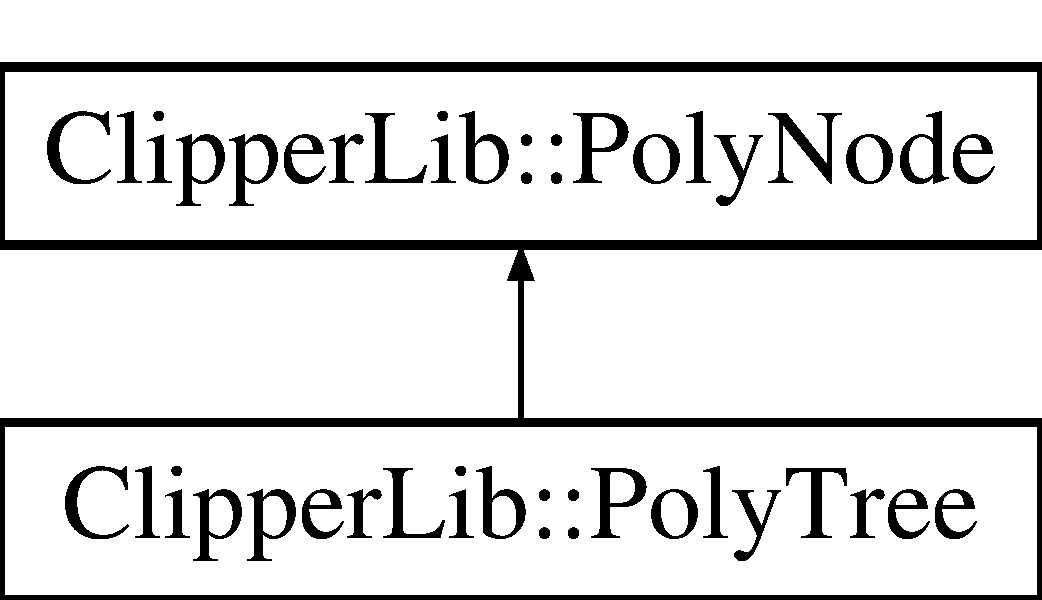
\includegraphics[height=2.000000cm]{classClipperLib_1_1PolyNode}
\end{center}
\end{figure}
\subsection*{Public Member Functions}
\begin{DoxyCompactItemize}
\item 
\hypertarget{classClipperLib_1_1PolyNode_ae9a4f50a1c9aec06c083578742d24bb7}{\hyperlink{classClipperLib_1_1PolyNode}{Poly\-Node} $\ast$ {\bfseries Get\-Next} () const }\label{classClipperLib_1_1PolyNode_ae9a4f50a1c9aec06c083578742d24bb7}

\item 
\hypertarget{classClipperLib_1_1PolyNode_aef7847f53087207b6e341c029adc1768}{bool {\bfseries Is\-Hole} () const }\label{classClipperLib_1_1PolyNode_aef7847f53087207b6e341c029adc1768}

\item 
\hypertarget{classClipperLib_1_1PolyNode_a76c8c55a45651cf3b5a67b8634173de8}{int {\bfseries Child\-Count} () const }\label{classClipperLib_1_1PolyNode_a76c8c55a45651cf3b5a67b8634173de8}

\end{DoxyCompactItemize}
\subsection*{Public Attributes}
\begin{DoxyCompactItemize}
\item 
\hypertarget{classClipperLib_1_1PolyNode_acb497b5e354eedbb5aa29531a1a57714}{Polygon {\bfseries Contour}}\label{classClipperLib_1_1PolyNode_acb497b5e354eedbb5aa29531a1a57714}

\item 
\hypertarget{classClipperLib_1_1PolyNode_a7ac59aea508951a4c979bfca8913261d}{Poly\-Nodes {\bfseries Childs}}\label{classClipperLib_1_1PolyNode_a7ac59aea508951a4c979bfca8913261d}

\item 
\hypertarget{classClipperLib_1_1PolyNode_a9465bc02623316de2af3ab52c6f7041e}{\hyperlink{classClipperLib_1_1PolyNode}{Poly\-Node} $\ast$ {\bfseries Parent}}\label{classClipperLib_1_1PolyNode_a9465bc02623316de2af3ab52c6f7041e}

\end{DoxyCompactItemize}
\subsection*{Friends}
\begin{DoxyCompactItemize}
\item 
\hypertarget{classClipperLib_1_1PolyNode_a4d39a09ecdddeeb85930dd4554a54b3c}{class {\bfseries Clipper}}\label{classClipperLib_1_1PolyNode_a4d39a09ecdddeeb85930dd4554a54b3c}

\end{DoxyCompactItemize}


The documentation for this class was generated from the following files\-:\begin{DoxyCompactItemize}
\item 
model/clipper/clipper.\-hpp\item 
model/clipper/clipper.\-cpp\end{DoxyCompactItemize}

\hypertarget{classClipperLib_1_1PolyOffsetBuilder}{\section{Clipper\-Lib\-:\-:Poly\-Offset\-Builder Class Reference}
\label{classClipperLib_1_1PolyOffsetBuilder}\index{Clipper\-Lib\-::\-Poly\-Offset\-Builder@{Clipper\-Lib\-::\-Poly\-Offset\-Builder}}
}
\subsection*{Public Member Functions}
\begin{DoxyCompactItemize}
\item 
\hypertarget{classClipperLib_1_1PolyOffsetBuilder_a5b0a249738e8093fa176d4ca2da1b1d9}{{\bfseries Poly\-Offset\-Builder} (const Polygons \&in\-\_\-polys, Polygons \&out\-\_\-polys, double delta, Join\-Type jointype, double limit, bool auto\-Fix)}\label{classClipperLib_1_1PolyOffsetBuilder_a5b0a249738e8093fa176d4ca2da1b1d9}

\end{DoxyCompactItemize}


The documentation for this class was generated from the following file\-:\begin{DoxyCompactItemize}
\item 
model/clipper/clipper.\-cpp\end{DoxyCompactItemize}

\hypertarget{classClipperLib_1_1PolyTree}{\section{Clipper\-Lib\-:\-:Poly\-Tree Class Reference}
\label{classClipperLib_1_1PolyTree}\index{Clipper\-Lib\-::\-Poly\-Tree@{Clipper\-Lib\-::\-Poly\-Tree}}
}
Inheritance diagram for Clipper\-Lib\-:\-:Poly\-Tree\-:\begin{figure}[H]
\begin{center}
\leavevmode
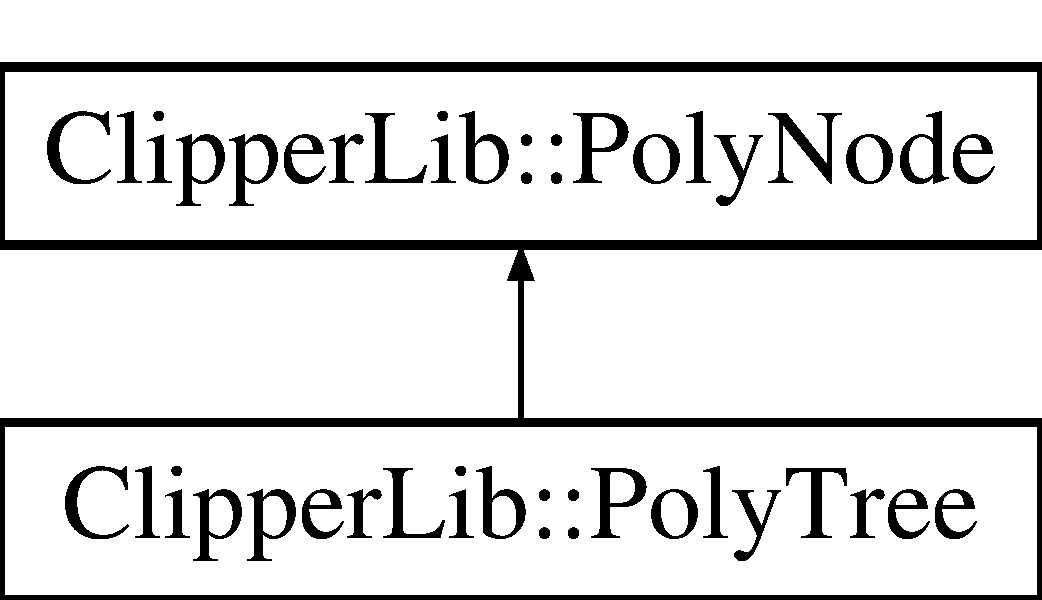
\includegraphics[height=2.000000cm]{classClipperLib_1_1PolyTree}
\end{center}
\end{figure}
\subsection*{Public Member Functions}
\begin{DoxyCompactItemize}
\item 
\hypertarget{classClipperLib_1_1PolyTree_ab678adb646c636e1f7a13e56cdc5bb93}{\hyperlink{classClipperLib_1_1PolyNode}{Poly\-Node} $\ast$ {\bfseries Get\-First} () const }\label{classClipperLib_1_1PolyTree_ab678adb646c636e1f7a13e56cdc5bb93}

\item 
\hypertarget{classClipperLib_1_1PolyTree_a8620ea631d478b3c43274ac084902ec4}{void {\bfseries Clear} ()}\label{classClipperLib_1_1PolyTree_a8620ea631d478b3c43274ac084902ec4}

\item 
\hypertarget{classClipperLib_1_1PolyTree_a28951d9ee7046c57388c7ddcbb3dcb6d}{int {\bfseries Total} () const }\label{classClipperLib_1_1PolyTree_a28951d9ee7046c57388c7ddcbb3dcb6d}

\end{DoxyCompactItemize}
\subsection*{Friends}
\begin{DoxyCompactItemize}
\item 
\hypertarget{classClipperLib_1_1PolyTree_a4d39a09ecdddeeb85930dd4554a54b3c}{class {\bfseries Clipper}}\label{classClipperLib_1_1PolyTree_a4d39a09ecdddeeb85930dd4554a54b3c}

\end{DoxyCompactItemize}
\subsection*{Additional Inherited Members}


The documentation for this class was generated from the following files\-:\begin{DoxyCompactItemize}
\item 
model/clipper/clipper.\-hpp\item 
model/clipper/clipper.\-cpp\end{DoxyCompactItemize}

\input{classmodel_1_1position}
\input{classmodel_1_1ProbFormula}
\input{classmodel_1_1Region}
\hypertarget{structClipperLib_1_1Scanbeam}{\section{Clipper\-Lib\-:\-:Scanbeam Struct Reference}
\label{structClipperLib_1_1Scanbeam}\index{Clipper\-Lib\-::\-Scanbeam@{Clipper\-Lib\-::\-Scanbeam}}
}
\subsection*{Public Attributes}
\begin{DoxyCompactItemize}
\item 
\hypertarget{structClipperLib_1_1Scanbeam_a71e4ab9957d1039c6d6666b92236fb71}{long64 {\bfseries Y}}\label{structClipperLib_1_1Scanbeam_a71e4ab9957d1039c6d6666b92236fb71}

\item 
\hypertarget{structClipperLib_1_1Scanbeam_a7e77b169ceff6cd0e079dd0e0b5760e8}{\hyperlink{structClipperLib_1_1Scanbeam}{Scanbeam} $\ast$ {\bfseries next}}\label{structClipperLib_1_1Scanbeam_a7e77b169ceff6cd0e079dd0e0b5760e8}

\end{DoxyCompactItemize}


The documentation for this struct was generated from the following file\-:\begin{DoxyCompactItemize}
\item 
model/clipper/clipper.\-hpp\end{DoxyCompactItemize}

\input{classmodel_1_1Segment}
\input{classmodel_1_1slice}
\input{classmodel_1_1stack}
\input{structmodel_1_1State__tag}
\input{structmodel_1_1StateProbAlt__tag}
\input{structmodel_1_1StateTimeAlt__tag}
\input{classSTDDialogController}
\input{structmodel_1_1StochasticEvent}
\hypertarget{structClipperLib_1_1TEdge}{\section{Clipper\-Lib\-:\-:T\-Edge Struct Reference}
\label{structClipperLib_1_1TEdge}\index{Clipper\-Lib\-::\-T\-Edge@{Clipper\-Lib\-::\-T\-Edge}}
}
\subsection*{Public Attributes}
\begin{DoxyCompactItemize}
\item 
\hypertarget{structClipperLib_1_1TEdge_a42d3306a851df6869a85f68495a1c4a3}{long64 {\bfseries xbot}}\label{structClipperLib_1_1TEdge_a42d3306a851df6869a85f68495a1c4a3}

\item 
\hypertarget{structClipperLib_1_1TEdge_a5cca9ccc325b346dc2a25001c4291f2a}{long64 {\bfseries ybot}}\label{structClipperLib_1_1TEdge_a5cca9ccc325b346dc2a25001c4291f2a}

\item 
\hypertarget{structClipperLib_1_1TEdge_a26717c33477dbe350518cd0819a9e3c6}{long64 {\bfseries xcurr}}\label{structClipperLib_1_1TEdge_a26717c33477dbe350518cd0819a9e3c6}

\item 
\hypertarget{structClipperLib_1_1TEdge_a075c45d9ae5c1d2d0a22a4778c2f7c74}{long64 {\bfseries ycurr}}\label{structClipperLib_1_1TEdge_a075c45d9ae5c1d2d0a22a4778c2f7c74}

\item 
\hypertarget{structClipperLib_1_1TEdge_ad171f585c0d88630f35fc87706ae1fde}{long64 {\bfseries xtop}}\label{structClipperLib_1_1TEdge_ad171f585c0d88630f35fc87706ae1fde}

\item 
\hypertarget{structClipperLib_1_1TEdge_a56b854b6224c1f0fc7903d5448229a3a}{long64 {\bfseries ytop}}\label{structClipperLib_1_1TEdge_a56b854b6224c1f0fc7903d5448229a3a}

\item 
\hypertarget{structClipperLib_1_1TEdge_aab44ea427e3da1631c15e1ff7c913108}{double {\bfseries dx}}\label{structClipperLib_1_1TEdge_aab44ea427e3da1631c15e1ff7c913108}

\item 
\hypertarget{structClipperLib_1_1TEdge_ab27923f96c12e80a3e6c95776333c811}{long64 {\bfseries delta\-X}}\label{structClipperLib_1_1TEdge_ab27923f96c12e80a3e6c95776333c811}

\item 
\hypertarget{structClipperLib_1_1TEdge_a103279aab6bb41f5c0672b9a7b79014b}{long64 {\bfseries delta\-Y}}\label{structClipperLib_1_1TEdge_a103279aab6bb41f5c0672b9a7b79014b}

\item 
\hypertarget{structClipperLib_1_1TEdge_a4ec20b0f419c70c81d57d3e1da27daf6}{long64 {\bfseries tmp\-X}}\label{structClipperLib_1_1TEdge_a4ec20b0f419c70c81d57d3e1da27daf6}

\item 
\hypertarget{structClipperLib_1_1TEdge_abcbfff8dad739351094a02487e59f4e7}{Poly\-Type {\bfseries poly\-Type}}\label{structClipperLib_1_1TEdge_abcbfff8dad739351094a02487e59f4e7}

\item 
\hypertarget{structClipperLib_1_1TEdge_a2024ade454223f57339ab6045d182e55}{Edge\-Side {\bfseries side}}\label{structClipperLib_1_1TEdge_a2024ade454223f57339ab6045d182e55}

\item 
\hypertarget{structClipperLib_1_1TEdge_a2e5b86c66d319f01e32b5d06596e36fb}{int {\bfseries wind\-Delta}}\label{structClipperLib_1_1TEdge_a2e5b86c66d319f01e32b5d06596e36fb}

\item 
\hypertarget{structClipperLib_1_1TEdge_a24e0e2bd7a90676c7a7ad5e2052878ed}{int {\bfseries wind\-Cnt}}\label{structClipperLib_1_1TEdge_a24e0e2bd7a90676c7a7ad5e2052878ed}

\item 
\hypertarget{structClipperLib_1_1TEdge_a803d452baf10e1cd5f5e17f758b298df}{int {\bfseries wind\-Cnt2}}\label{structClipperLib_1_1TEdge_a803d452baf10e1cd5f5e17f758b298df}

\item 
\hypertarget{structClipperLib_1_1TEdge_a63e563de2857398a9c8b0d4904679d84}{int {\bfseries out\-Idx}}\label{structClipperLib_1_1TEdge_a63e563de2857398a9c8b0d4904679d84}

\item 
\hypertarget{structClipperLib_1_1TEdge_a21c3dba96acc90b5bc00ca3db68445f6}{\hyperlink{structClipperLib_1_1TEdge}{T\-Edge} $\ast$ {\bfseries next}}\label{structClipperLib_1_1TEdge_a21c3dba96acc90b5bc00ca3db68445f6}

\item 
\hypertarget{structClipperLib_1_1TEdge_ac81ef1c52f20b36b321d2a9208f97389}{\hyperlink{structClipperLib_1_1TEdge}{T\-Edge} $\ast$ {\bfseries prev}}\label{structClipperLib_1_1TEdge_ac81ef1c52f20b36b321d2a9208f97389}

\item 
\hypertarget{structClipperLib_1_1TEdge_af9f1d12d9a024e0aeb0a5810e66a343d}{\hyperlink{structClipperLib_1_1TEdge}{T\-Edge} $\ast$ {\bfseries next\-In\-L\-M\-L}}\label{structClipperLib_1_1TEdge_af9f1d12d9a024e0aeb0a5810e66a343d}

\item 
\hypertarget{structClipperLib_1_1TEdge_a2e4f5e8ffce918c2d5cf260252a4e811}{\hyperlink{structClipperLib_1_1TEdge}{T\-Edge} $\ast$ {\bfseries next\-In\-A\-E\-L}}\label{structClipperLib_1_1TEdge_a2e4f5e8ffce918c2d5cf260252a4e811}

\item 
\hypertarget{structClipperLib_1_1TEdge_a0da02ede8e83c3a4b27a09ebde1dfcf3}{\hyperlink{structClipperLib_1_1TEdge}{T\-Edge} $\ast$ {\bfseries prev\-In\-A\-E\-L}}\label{structClipperLib_1_1TEdge_a0da02ede8e83c3a4b27a09ebde1dfcf3}

\item 
\hypertarget{structClipperLib_1_1TEdge_aa98ac28e25e2a0bf4001ca9547ea0ae8}{\hyperlink{structClipperLib_1_1TEdge}{T\-Edge} $\ast$ {\bfseries next\-In\-S\-E\-L}}\label{structClipperLib_1_1TEdge_aa98ac28e25e2a0bf4001ca9547ea0ae8}

\item 
\hypertarget{structClipperLib_1_1TEdge_aead630eae0633921989272f74d7d169b}{\hyperlink{structClipperLib_1_1TEdge}{T\-Edge} $\ast$ {\bfseries prev\-In\-S\-E\-L}}\label{structClipperLib_1_1TEdge_aead630eae0633921989272f74d7d169b}

\end{DoxyCompactItemize}


The documentation for this struct was generated from the following file\-:\begin{DoxyCompactItemize}
\item 
model/clipper/clipper.\-hpp\end{DoxyCompactItemize}

\input{classmodel_1_1TimedDiagram}
\input{structToken}
\input{structmodel_1_1Transition}
\input{classmodel_1_1TrueFormula}
\input{classmodel_1_1UntilFormula}
\input{structyy__buffer__state}
\input{structyy__trans__info}
\input{unionyyalloc}
\input{unionYYMINORTYPE}
\input{structyyParser}
\input{structyyStackEntry}
\input{unionYYSTYPE}
\input{unionyystype}
\chapter{File Documentation}
\input{Facade_8cpp}
\input{fmll_8cpp}
\input{fmly_8cpp}
\input{location_8hh}
\input{position_8hh}
\input{ModelChecker_8cpp}
\addcontentsline{toc}{part}{Index}
\printindex
\end{document}
